%%
% TUM Corporate Design LaTeX Templates
% Based on the templates from https://www.tum.de/cd
%
% Feel free to join development on
% https://gitlab.lrz.de/tum-templates/templates
% and/or to create an issue in case of trouble.
%
% tum-presentation class for scientific talks, thesis presentations, ...
%
%%

%\documentclass[4to3]{tum-presentation}
%\documentclass[navsym]{tum-presentation}
%\documentclass[nothreeliner]{tum-presentation}
%\documentclass[handout,4on1]{tum-presentation}
%\documentclass[handout,2on1]{tum-presentation}
%\documentclass[handout]{tum-presentation}
\documentclass{tum-presentation}
\usepackage[font=small,labelfont=bf]{caption}
\usepackage{subcaption}
\usepackage{floatrow}
\usepackage{graphicx}
\usepackage[showframe]{geometry}
\addbibresource{literature.bib}

\title[Shortened Title]{Clustering-Based Sentiment Analysis for Media Agenda Setting}
\subtitle{Opinion Lab Group 2.3, presentation 5}
\author{Wing Sheung Leung, Qiaoxi Liu}
%\institute[]{\inst{1} Department of Electrical and Computer Engineering,
%  Technical University of Munich (TUM)\\
%  \inst{2} Department of Informatics, Technical University of Munich (TUM)}
%\date{International Conference on Mostly Scientific Topics}

\footline{\insertshortauthor~| \inserttitle}

\begin{document}

\begin{frame}[noframenumbering]
  \titlepage
\end{frame}
\begin{frame}
  \frametitle{Milestones}
  \vspace{2cm}
 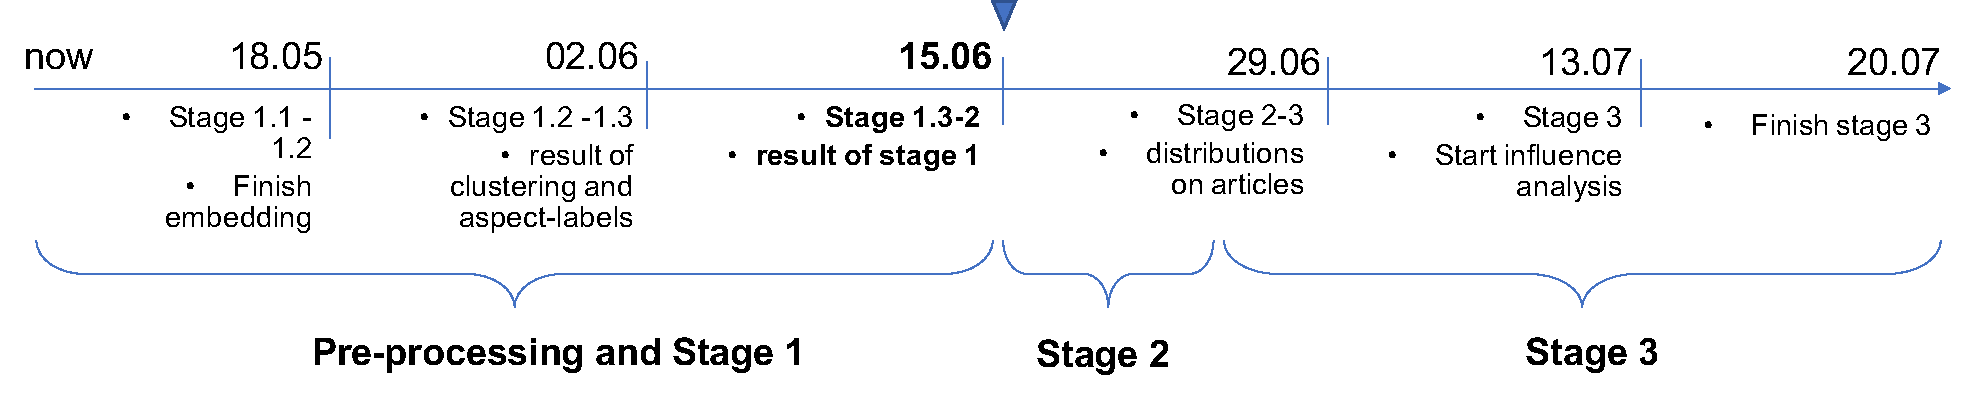
\includegraphics[width = \textwidth]{figures/timeline.pdf}
  
\end{frame}
\begin{frame}[t]
  \frametitle{Overview}
  \tableofcontents[sectionstyle=show,subsectionstyle=show,subsubsectionstyle=shaded]
\end{frame}



\section{Stage 1: Generate sentence embeddings with our corpus}
\subsection{1.1 Embeddings}
\subsubsection{XLING sentence-level embeddings}

\subsubsection{Indexing sentences}
\subsection{1.2 Kmeans and Elbow Method}
\subsubsection{sklearn.cluster.MiniBatchKMeans}
\subsubsection{Elbow Method for determining optimal k}

\subsection{1.3 Identifying topics and setting sentiment}
\subsubsection{Generate topword list}%ClarityscoreGenerator vs. word frequency
\subsubsection{Extracting topics form clustering results}
\subsubsection{Assigning sentiment by pre-trained model}


\begin{frame}
  \frametitle{Output from stage 1}
    
  \begin{figure}[t]
    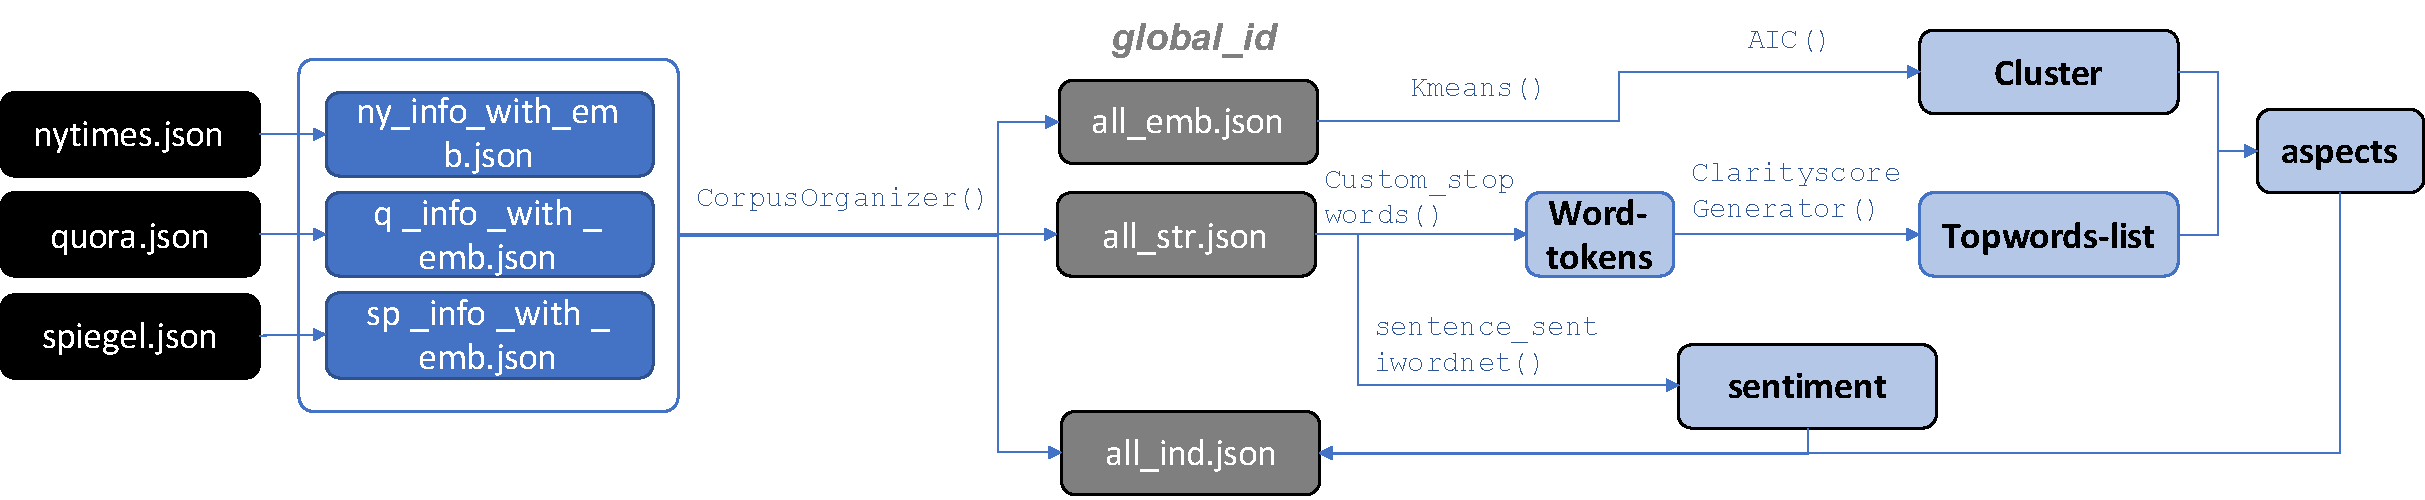
\includegraphics[width = \textwidth]{figures/journey.pdf}
    \end{figure}

\begin{tabular}{lrlrrlrr}
  {} &  global\_id & corpus\_name &  doc\_id &  com\_id &        date &  cluster &  sentiment \\
  
  0 &          0 &     nytimes &       0 &     NaN &  2005-11-01 &        7 &    0.12500 \\
  1 &          1 &     nytimes &       0 &     NaN &  2005-11-01 &        7 &   -0.12500 \\
  2 &          2 &     nytimes &       0 &     NaN &  2005-11-01 &        9 &    0.07500 \\
  3 &          3 &     nytimes &       0 &     NaN &  2005-11-01 &        7 &    0.50000 \\
  4 &          4 &     nytimes &       0 &     NaN &  2005-11-01 &        7 &   -0.03125 \\
 
  \end{tabular}
\end{frame}

\section{Stage 2: Distribution}

\begin{frame}
  \frametitle{Stage 2: Distribution of articles and comments Overview }
  \framesubtitle{Comments from NYTimes and Spiegel }
  \begin{description}
 \large
 \item NYtimes
    \item 99 out of 327 news have comments.
    \item Number of sentences among comments from each news:
    \item \begin{itemize}
      \item minmax = (3, 2535)
      \item mean = 481.7
      \item median= 216.0
    \end{itemize}
  \end{description}
  \vspace{0.7cm}
  \begin{description}
    \large
    \item Spiegel
       \item 61 out of 152 news have comments.
       \item Number of sentences among comments from each news:
       \item \begin{itemize}
         \item minmax=(8, 23255)
         \item mean = 2309.0
         \item median= 697.0
       \end{itemize}
     \end{description}
\end{frame}

\begin{frame}
  \frametitle{Sampling}
  \begin{description}
 \large
    \item To analyse the correlations between news and its comments, we select the news with more comments.
    \item \begin{itemize}
    \item NYtimes: selected 52 out of 99 news with comments (each news has 200+ sentences of comments)
    \item Spiegel: selected 34 out of 61 news with comments (each news has 500+ sentences of comments)
  \end{itemize}
  \end{description}
\end{frame}

\begin{frame}[fragile]
  \frametitle{Statsitc on distirbution Approach 1  }
  \framesubtitle{Accumulating and Normalizing (separate positive and negative)}
  \begin{description}
    \large
    \item 1. accumulate positive$/$negative sentences from each tuple 
    \begin{lstlisting}
      cluster_group = doc.groupby('cluster')
      for (_,cluster) in cluster_group:
        label = cluster.cluster.unique()[0]
        doc_dic[label] = sum([abs(x) for x in scores]), sum([x for x in scores if x>0])
      \end{lstlisting}
      \item 2. normalize the accumulation score
    
      \begin{lstlisting}
        df_new_t['normalized_pos'] = (df_new_t[1])/all_abs_sum
        df_new_t['normalized_neg'] = (df_new_t[2])/all_abs_sum
  
    \end{lstlisting}
    \item Example:
    \small
    \begin{tabular}{lrr}
    
      {} &  normalized\_pos &  normalized\_neg \\
     
      Chemicals \& Cancer &        0.000000 &       -0.023515 \\
      Meat \& Animals     &        0.032921 &       -0.028218 \\
      Health \& Diet      &        0.000000 &       -0.009406 \\
      Retail             &        0.206930 &       -0.069604 \\
      GMO                &        0.157471 &       -0.289232 \\
      Agriculture        &        0.058858 &       -0.089356 \\
      Polices            &        0.031353 &        0.000000 \\
      Economy            &        0.003135 &        0.000000 \\
      
      \end{tabular}
  \end{description}
\end{frame}
\subsection{Representing sentiment distribution for single article}
\begin{frame}
  \frametitle{Representing NYTimes articles}
  \begin{columns}[t]
    \column{.5\textwidth}
    \centering
    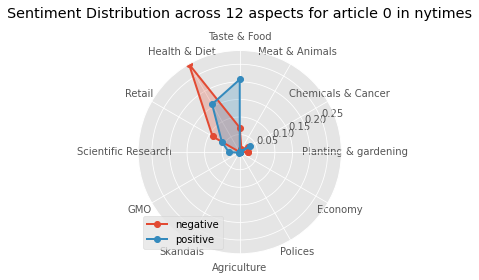
\includegraphics[width = \textwidth]{figures/radar_nytimes_0.png}\\
    \column{.5\textwidth}
    \centering
    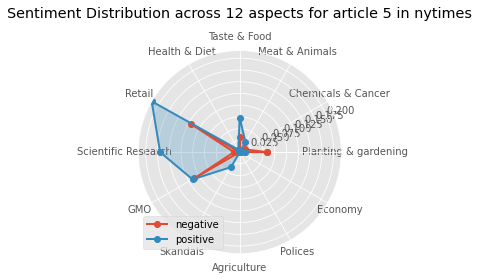
\includegraphics[width = \textwidth]{figures/radar_nytimes_5.png}
    \end{columns}
\end{frame}




\begin{frame}[fragile]
  \frametitle{Statsitc on distirbution Approach 2}
  \framesubtitle{Summing up all sentiment scores and average}
  \begin{description}
    \large

    \item 1.instead of accumulating separately, we sum up sentences from each cluster and use weights
    \begin{lstlisting}
      for (_,cluster) in cluster_group:
        label = cluster.cluster.unique()[0]
        scores = np.array(cluster['sentiment'])
      \end{lstlisting}
      \item 2. calculate weight and mean for each cluster
      
      \begin{lstlisting}
      df = pd.DataFrame(scores,columns=['scores'])
      df['weight'] = length_per_cluster/total_num_sen
      df['mean'] = scores.mean()
    \end{lstlisting}
    \item 3. remove 0 score sentences in German comments ("Zitat von")
    \item 4. boxplot
    \begin{lstlisting}
      ggplot(aes(y=scores,factor(cluster),fill=mean,weight=weight))
    \end{lstlisting}

    \item  \begin{itemize}
      \item color = mean of sentiment scores
    \item wider = more weight (thinner = less weight)
    
    \item higher = larger variance (flatter = smaller 
    variance)
    \end{itemize}
  \end{description}
\end{frame}

\begin{frame}
  \frametitle{NYTimes: Labeling GMO}
  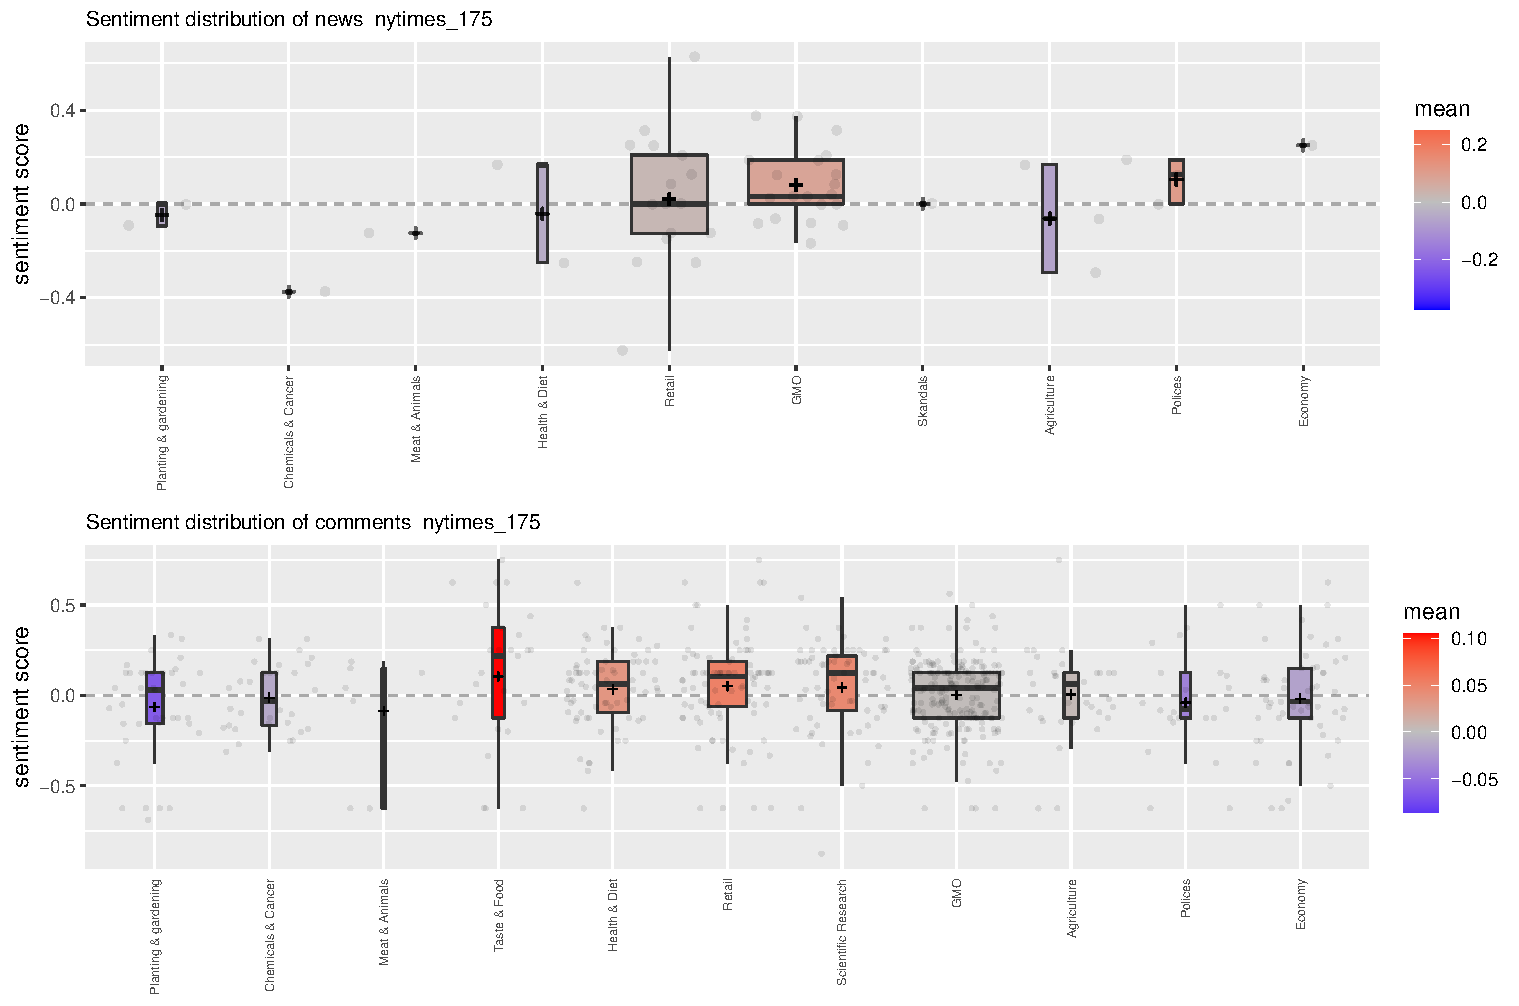
\includegraphics[width =0.65 \textwidth]{figures/boxplot_nytimes_175.pdf}
  
\end{frame}

\begin{frame}
  \frametitle{NYTimes: Labeling GMO}
  \begin{description}
    \item \textbf{article}:
    \item Whole Foods Market, the grocery chain, on Friday became the first retailer in the United States to require labeling of all genetically modified foods sold in its stores, a move that some experts said could radically alter the food industry. ... Whole Foods, which specializes in organic products, tends to be favored by those types of consumers, and it enjoys strong sales of its private-label products, whose composition it controls. ... He said Whole Foods looked forward to working with suppliers on the labeling.
    \item \textbf{comments}:
    \item  \begin{itemize}
    \item Sometimes genetically modifying food has unintended consequences like bad tasting tomatoes (or worse)
    \item I have a cousin who works at Whole Foods. He is a happy employee and loves it. Thinks it is a great company.
    \item I am not sure if non-GMO foods are healthier to eat but they are certainly better for the environment.
    \item I applaud Whole Foods for at least taking a stand.
    \item consuming red meat is an emotionally charged issue for many people.
    \item In March 2012, Harvard Public Health published the results of a study on red meat, which followed 120,000 people over 20 years. The conclusion: "Red meat consumption is associated with an increased risk of total, heart, and cancer mortality"
    \item Since apples are apparently the most pesticide-ridden fruit, I have gotten to like the more expensive but sweeter ones.
  \end{itemize}
   \end{description}
\end{frame}
\begin{frame}
  \frametitle{Spiegel: 5\% Spielraum von Bionade }
  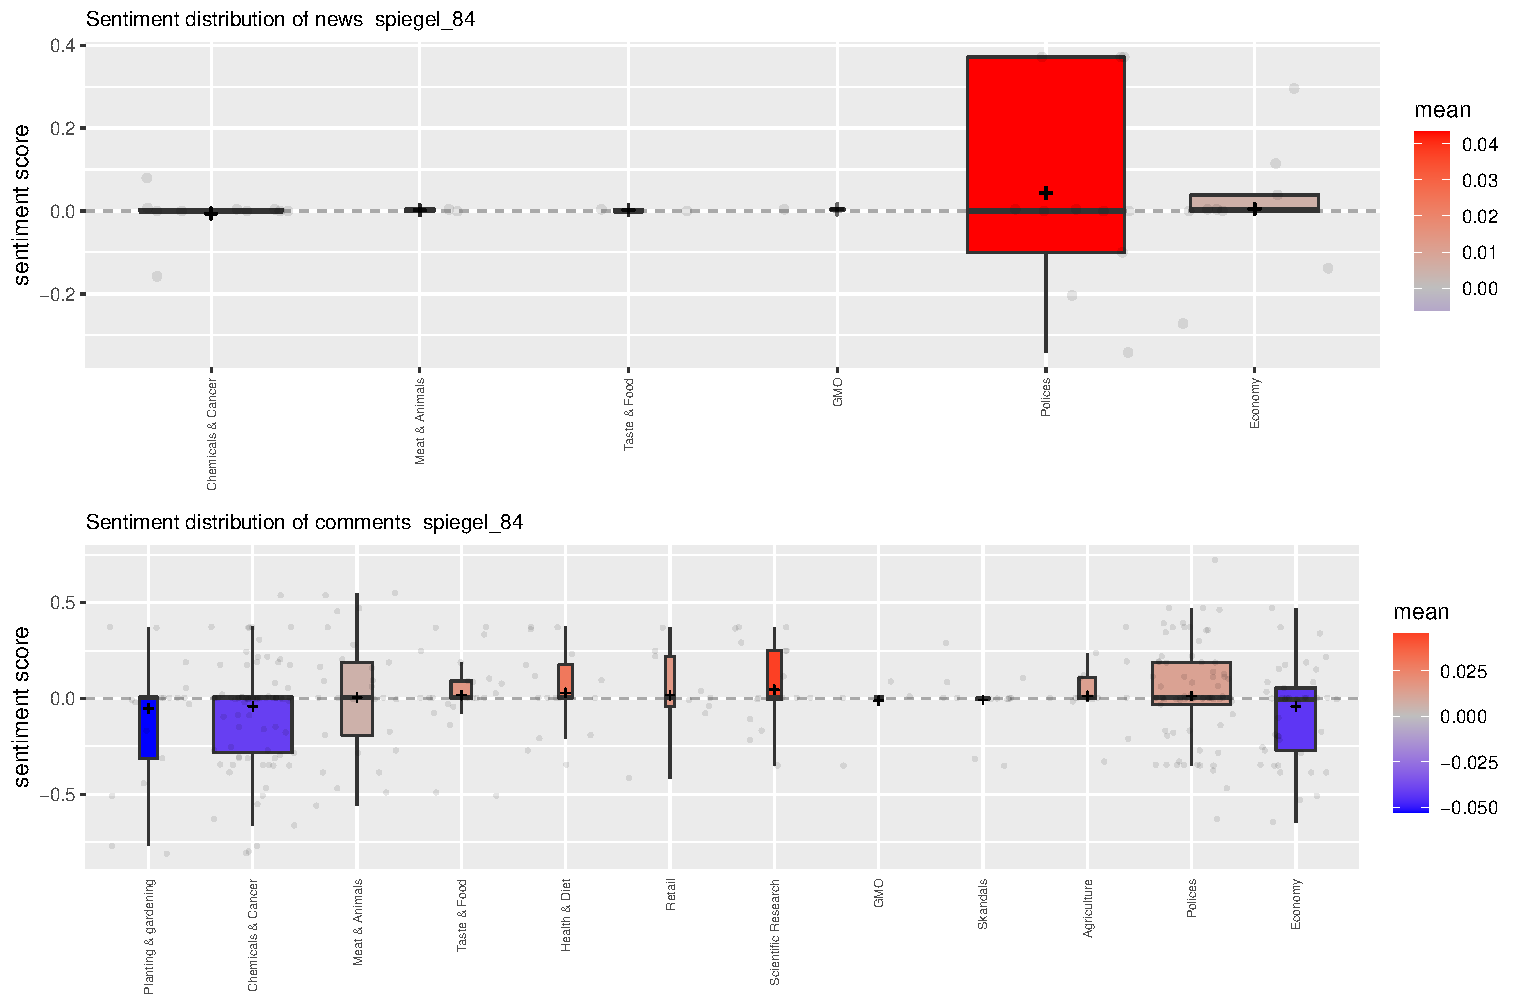
\includegraphics[width =0.65 \textwidth]{figures/boxplot_spiegel_84.pdf}
  
\end{frame}
\begin{frame}
  \frametitle{ Spiegel: 5\% Spielraum von Bionade }
  \begin{description}
    \item \textbf{article}:
    \item Es ist eine erstaunliche Erfolgsgeschichte: Kaum ein Produkt hat den Markt in kürzester Zeit so verändert wie Bionade, das Brausegetränk aus Bayern. Jetzt aber hat das Unternehmen Probleme, Bio-Rohstoffe zu bekommen - und zeigt damit, dass sich Öko-Anspruch und Wachstum nicht immer vertragen...."Bionade nutzt Spielraum aus". Möglich ist das, weil der Gesetzgeber den Produzenten beim Bio-Siegel eine Lücke gelassen hat. Wer das grün-schwarze EU-Zertifikat auf seine Produkte drucken will, der muss nur bei 95 Prozent der Zutaten nachweisen, dass sie biologisch angebaut sind. "Diesen Spielraum von fünf Prozent nutzt Bionade aus", sagt Markwardt.
    \item \textbf{comments}:
    \item  \begin{itemize}
    \item  Wie sollen Menschen in Deutschen Staedten Litschi anbauen ?...das Thema Biolebensmittel und Biolandwirtschaft viel zu komplex ist, ... Nur Städter am Schreibtisch können sich dafür begeistern,welche von Tierhaltung,Biologie,Ökologie nur Theoriewissen haben... Kaum jemand hat selbst mal Hühner gehalten geschweige denn Großtiere. ...Wer hat z.B.schon mal tatsächlich in der Landwirtschaft gearbeitet,Gemüse angebaut,Nutztiere gehalten ?doch kaum jemand! ...daß hier mal wirklich über WAS IST BIO diskutiert wird .
    \item Ich selbst habe mich maßlos über die unverschämte Preiserhöhung von Bionade geärgert.
    \item Möglichst billige Rohstoffe, möglichst billige Angestellte.
    \item Arbeitswirtschaftlich sind Bestände über 500 Tier ...bei den niedrigen Erzeugerpreisen nicht von Hand zu füttern. Zudem gibt es sehr viele (unabhängige) Untersuchungen die gerade in der Geflügelhaltung technische Hilfsmittel mit Blick auf die Tiergesundheit sowie die Tierbedürfnisse positiv bewerten.
    
  \end{itemize}
   \end{description}
\end{frame}
\begin{frame}
  \frametitle{Spiegel: Der Skandal um Dioxin }
  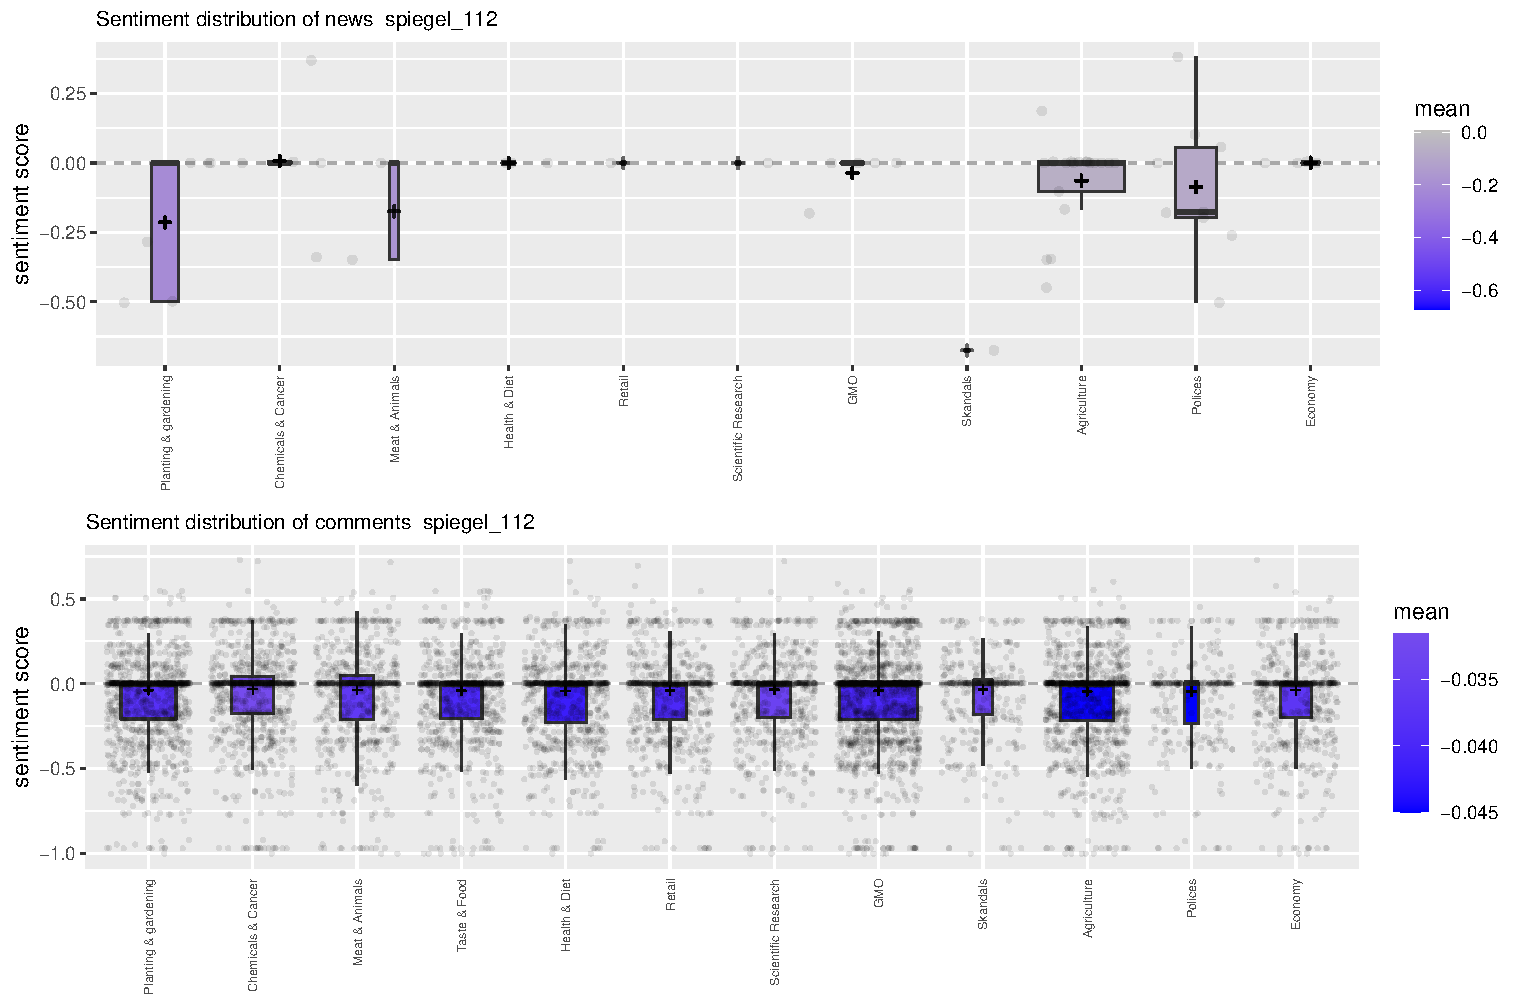
\includegraphics[width =0.65 \textwidth]{figures/boxplot_spiegel_112.pdf}
  
\end{frame}
\begin{frame}
  \frametitle{ Spiegel: 5\% Spielraum von Bionade }
  \begin{description}
    \item \textbf{article}:
    \item Es ist einer der größten Giftskandale der vergangenen Jahre: Bis zu 3000 Tonnen dioxinverseuchtes Fett wurden laut Bundeslandwirtschaftsministerium an 25 Futtermittelhersteller in mindestens vier Bundesländern geliefert. Wo das Gift von dort aus hingelangte und welche Mengen an Nahrungsmitteln belastet sind, ist weitgehend unklar. Verbraucher reagieren zunehmend verunsichert: Der Verkauf von Hühnereiern ist "spürbar" gesunken, teilte die landwirtschaftliche Marktberichterstattungsstelle MEG mit. Welche Gefahren drohen durch die Einnahme von Dioxin? Welche Vorsichtsmaßnahmen können getroffen werden? SPIEGEL ONLINE gibt Antworten auf sieben Fragen.
    \item \textbf{comments}:
    \item  \begin{itemize}
      \item  Der Dioxin-Skandal war hoffentlich nicht der letzte. Es sollten so viele wie möglich vorkommen. Am besten aber wäre, wenn ein paar Konsumenten nachweislich an solchen oder anderen Giftstoffen in Lebensmitteln sterben.
      \item 3000 Tonnen verseuchtes Tierfutter - das ist ein Terroranschlag.
      \item Ich kann und will niemandem verbieten Fleisch von deutschen Rindern zu essen.
      \item den gesetzlichen Vorgaben ist so eine Sache. Fahren Sie mal mit einem Fiat 500 mit 80 km/h frontal gegen eine S-Klasse!. Ihr Vergleich hinkt doch wohl. Wer sich mit Bio-Artikeln überfrisst, stirbt auch. Also sind Bio-Lebensmittel auch lebensgefährlich, wenn man falsch damit umgeht. Guten Appetit.
      
    \end{itemize}
   \end{description}
\end{frame}

\begin{frame}
  \frametitle{Manually observed Features}
 
  \begin{itemize}
    \item Spiegel
    \begin{itemize}
      \item news: Kritical (suspection) 
      \item comments:  Sarkasmus, irony, not direct, more philosophic, spreading among more topics ,
    \end{itemize}
    \item NYtimes
    \begin{itemize}
      \item news: More like an advertisment for stakeholder 
    \item comments: simpler, clear statement (against or for), benefit or not
      \end{itemize}
  \end{itemize}

\end{frame}


\begin{frame}
  \frametitle{Next Plan}
  \begin{itemize}
    \item To improve the visualization and capture more patterns
    \item To measure the influence of articles onto commenters using Granger coefficients and cross-lagged correlations
\end{itemize}
\end{frame}


\section{Re-examination on topwords and Kmeans}
\begin{frame}
  \frametitle{Re-examination on topwords and Kmeans}
    Original methodology
    \begin{enumerate}
      \item Kmean clustering on embeddings of both English and German text all together
      \item Find topwords with naive method, simple term-frequency count with NLTK and self-defined stopwords
      \item Find topwords with calculating clarity scoring \[score_a(w) = t_a(w) log_2\frac{t_a(w)}{t(w)}\], where $t_a(w)$ and $t(w)$ are the l1-normalized tf-idf scores of w in the segments annotated with aspect a (i.e. topic / cluster) and in all annotated segments
    \end{enumerate}
\end{frame}


\begin{frame}
  \frametitle{Re-examination on topwords and Kmeans}
    Second methodology
    \begin{enumerate}
      \item Kmean clustering on embeddings of both English and German text all together
      \item Calculate clarity scoring \textbf{\emph{separately for English and German content}} \[score_a(w_{language}) = t_a(w_{language}) log_2\frac{t_a(w_{language})}{t(w_{language})}\], where $t_a(w_{language})$ and $t(w_{language})$ are the l1-normalized tf-idf scores of w in the segments annotated with aspect a (i.e. topic / cluster) for a certain language and in all annotated segments in that langauage
      \item Pick 10 topwords with highest clarity score in each cluster of each language, total 20 words for a cluster
      \item Sort the words by their relative clarity scores
      \[RelativeClarityScore_{language} = \frac{score_{language, i}}{\sum_{i=1}^{n} score_{language, i}}\]
    \end{enumerate}
\end{frame}


\begin{frame}
  \frametitle{Re-examination on topwords and Kmeans}
    Additional try
    \begin{enumerate}
      \item Kmean clustering on embeddings of German text and English separately
      \item Find topwords with calculating clarity scoring \textbf{\emph{separately for German content and English content}} \[score_a(w_{language}) = t_a(w_{language}) log_2\frac{t_a(w_{language})}{t(w_{language})}\], where $t_a(w_{language})$ and $t(w_{language})$ are the l1-normalized tf-idf scores of w in the segments annotated with aspect a (i.e. topic / cluster) for a certain language and in all annotated segments in that langauage
    \end{enumerate}
\end{frame}

\begin{frame}
    \vspace{4cm}
    \centering
    \Large{Appendix}
\end{frame}

\begin{figure}
\floatsetup{capposition = below, floatrowsep =qquad,}
\begin{subfloatrow}
    \ffigbox[\textwidth]{\caption{\small{Original methodology: naive method via simple term-frequency count}}}{%
  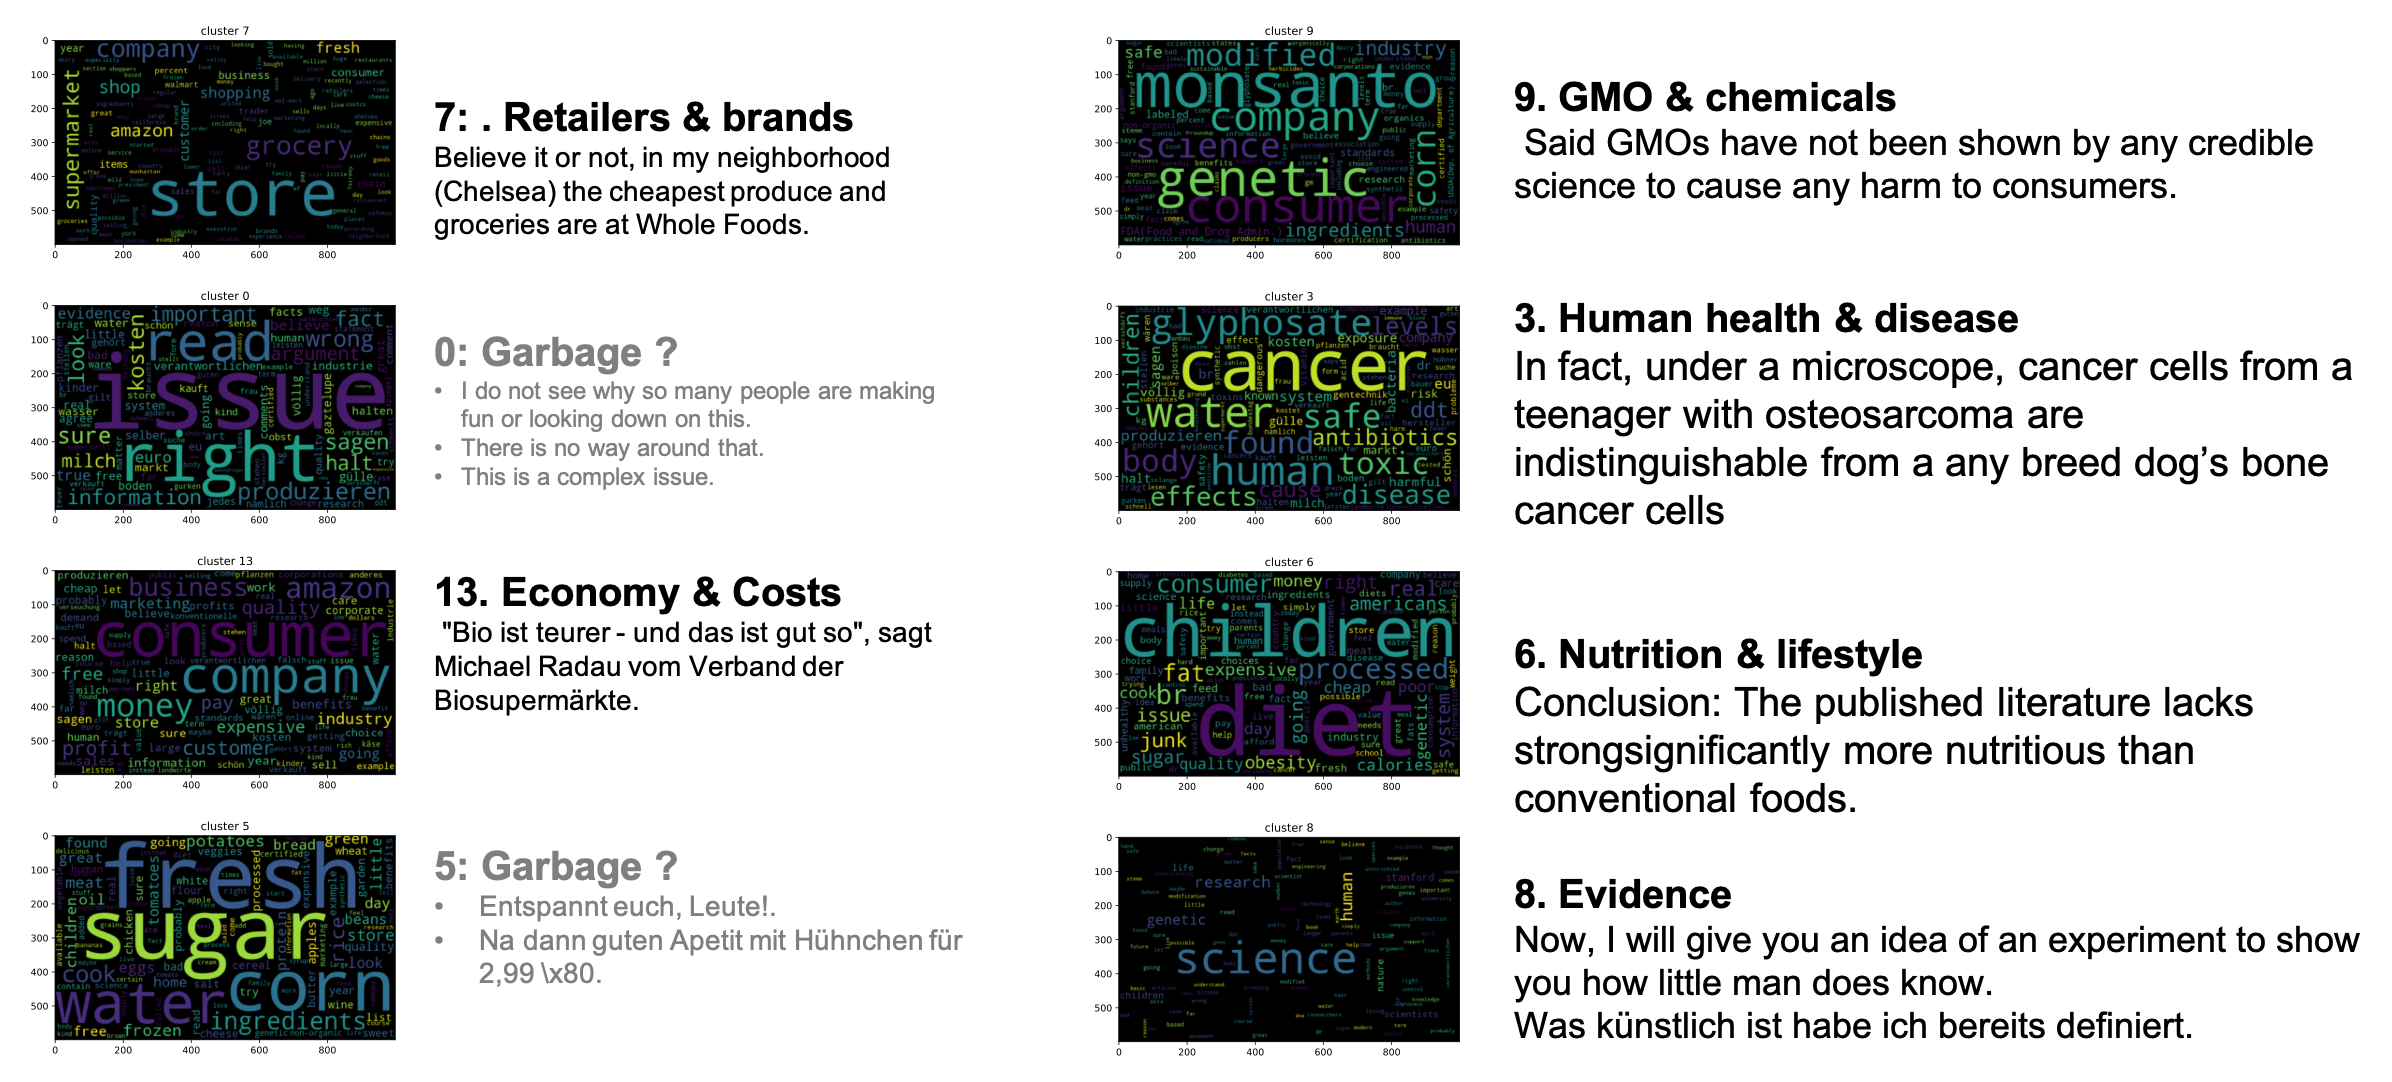
\includegraphics[width=0.4\textwidth]{figures/example16_1.png}%
  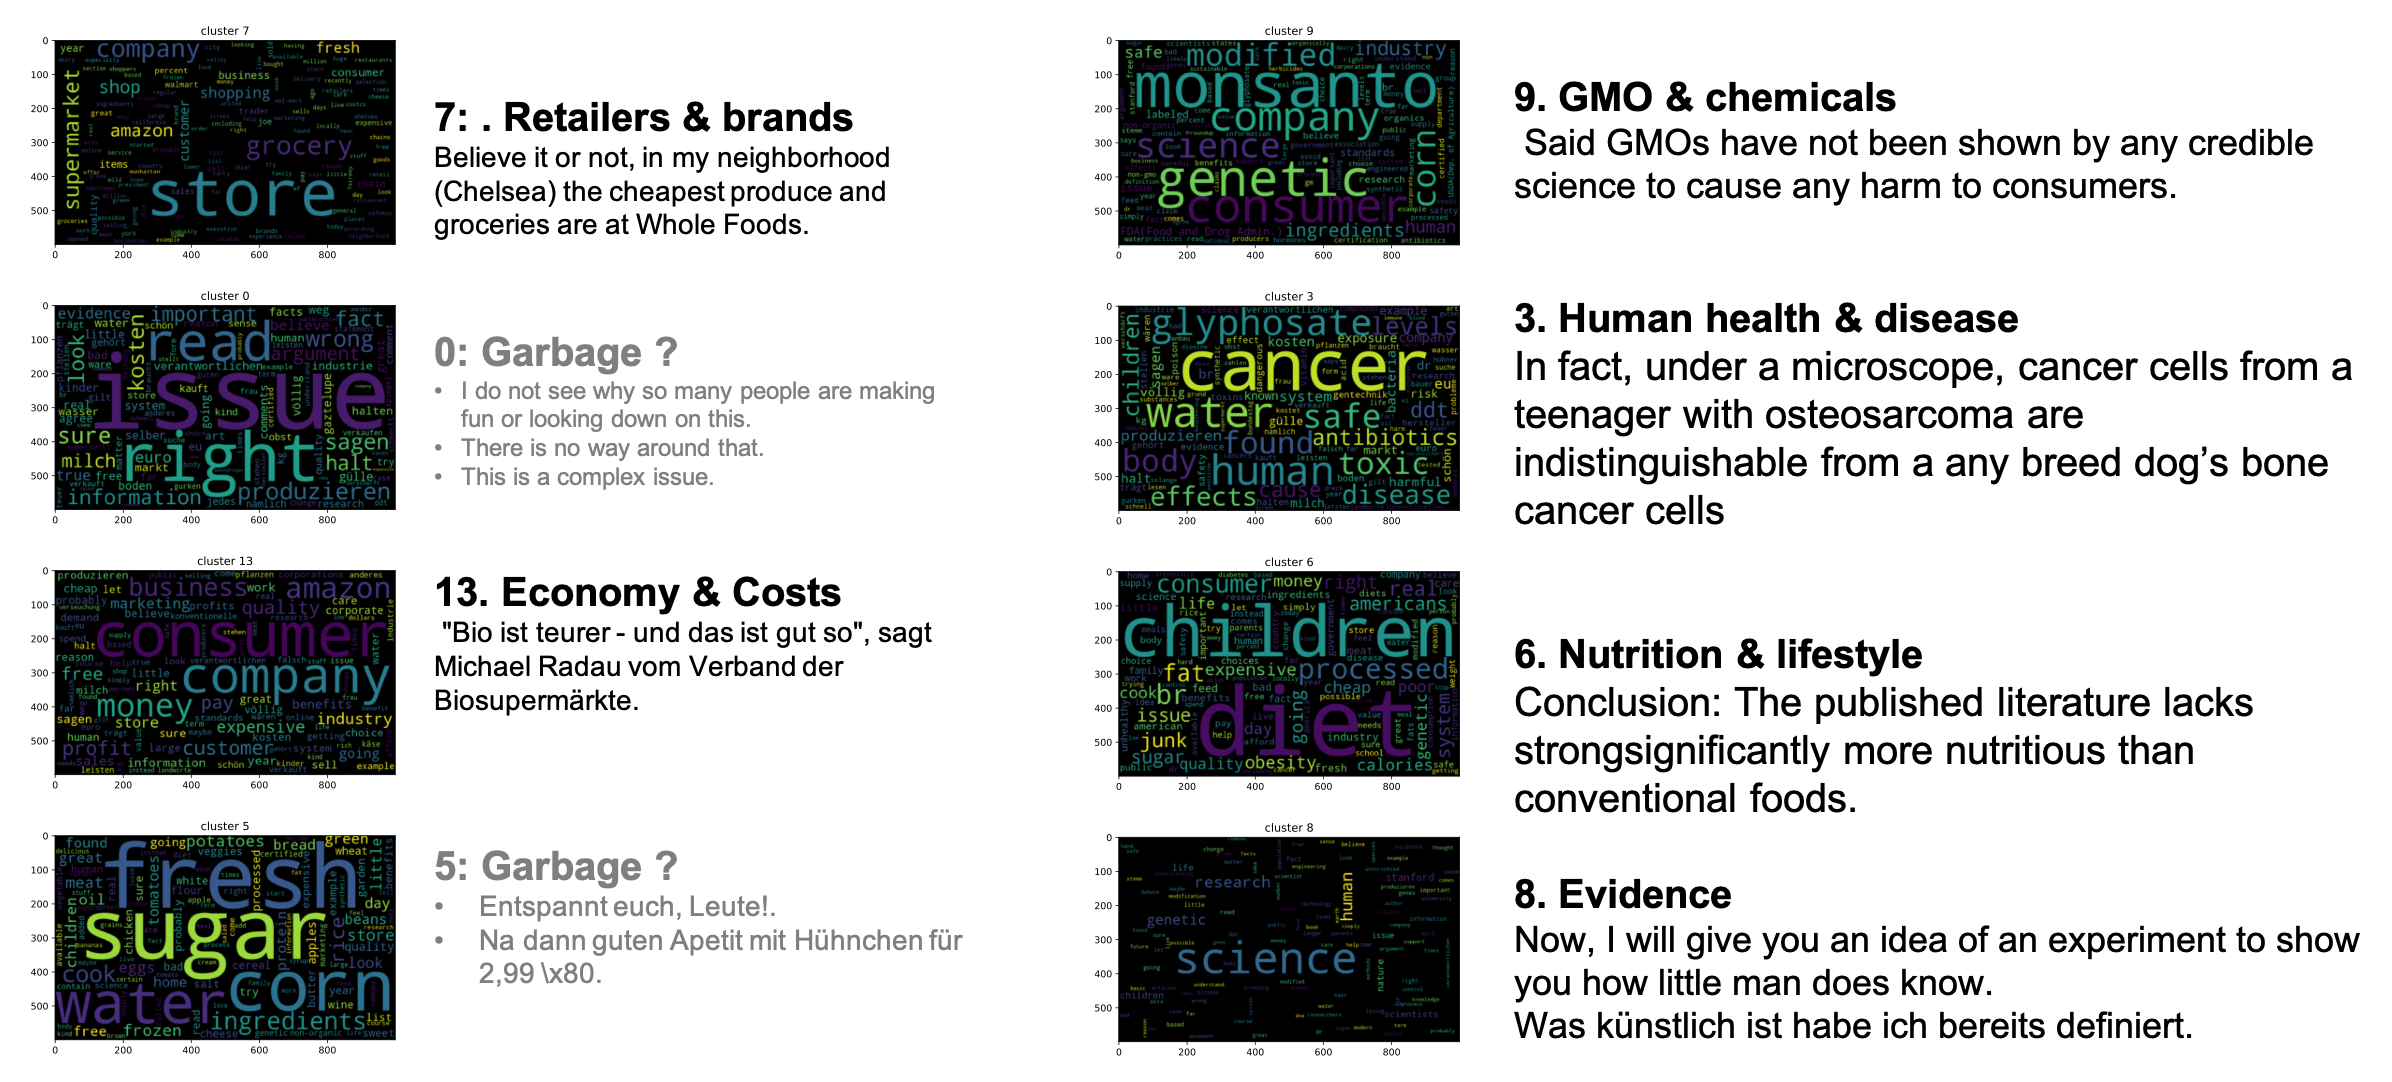
\includegraphics[width=0.4\textwidth]{figures/example16_1.png}%him
  }
\end{subfloatrow}
\begin{subfloatrow}
    \ffigbox[0.5\textwidth]{\caption{\small{Original methodology: clarity scores with NLTK and sklearn stopwords}}}{%
  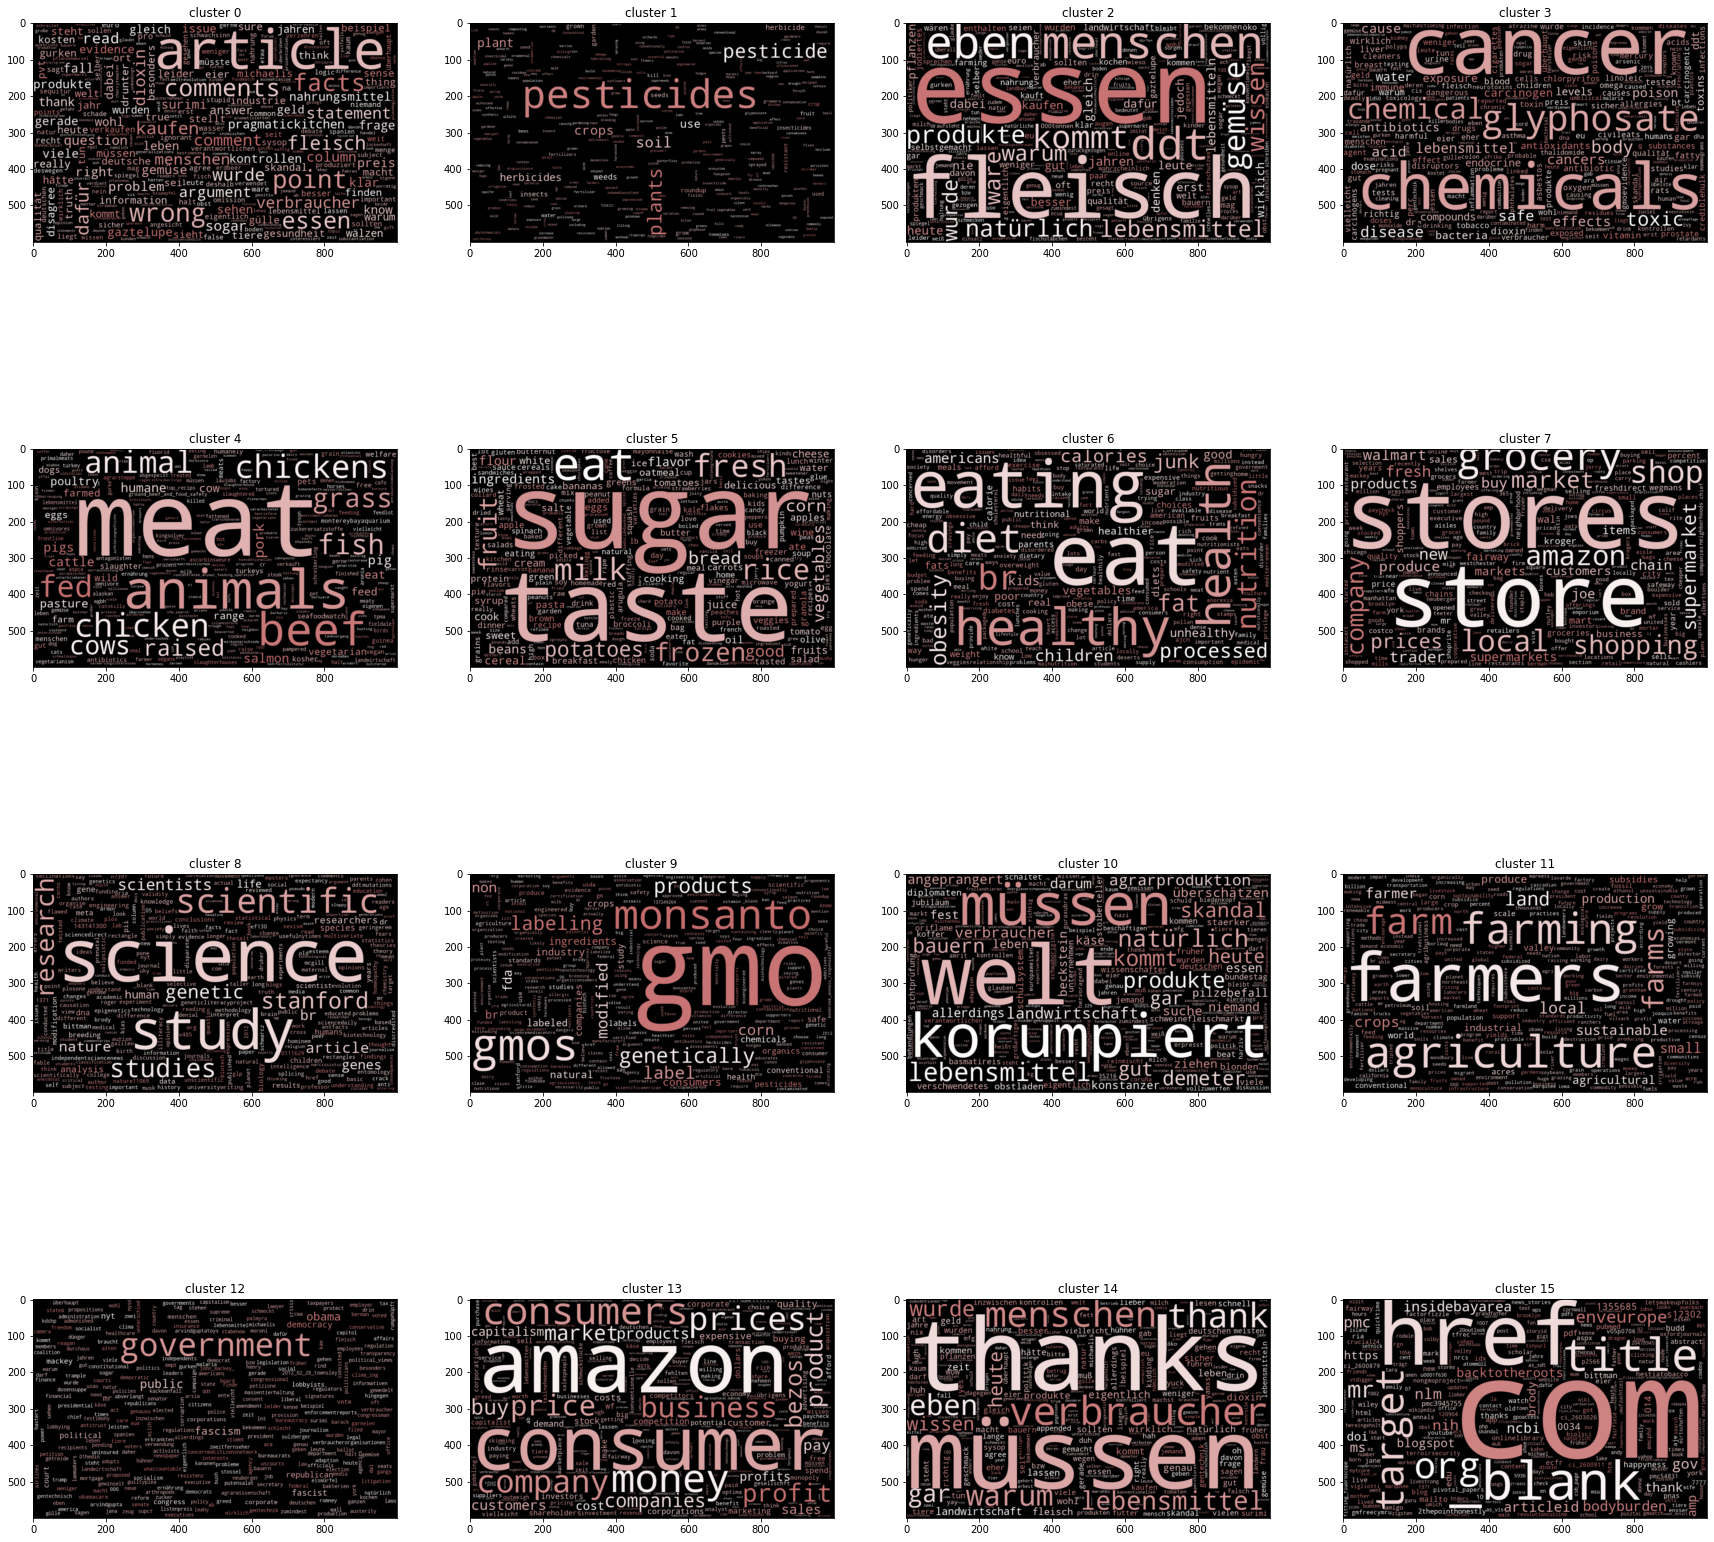
\includegraphics[width=0.3\textwidth]{images/nltk_sklearn_wordcloud_with_full_features.png}%
  }
    \ffigbox[0.5\textwidth]{\caption{\small{Original methodology: clarity scores with TF-High stopwords}}}{%
  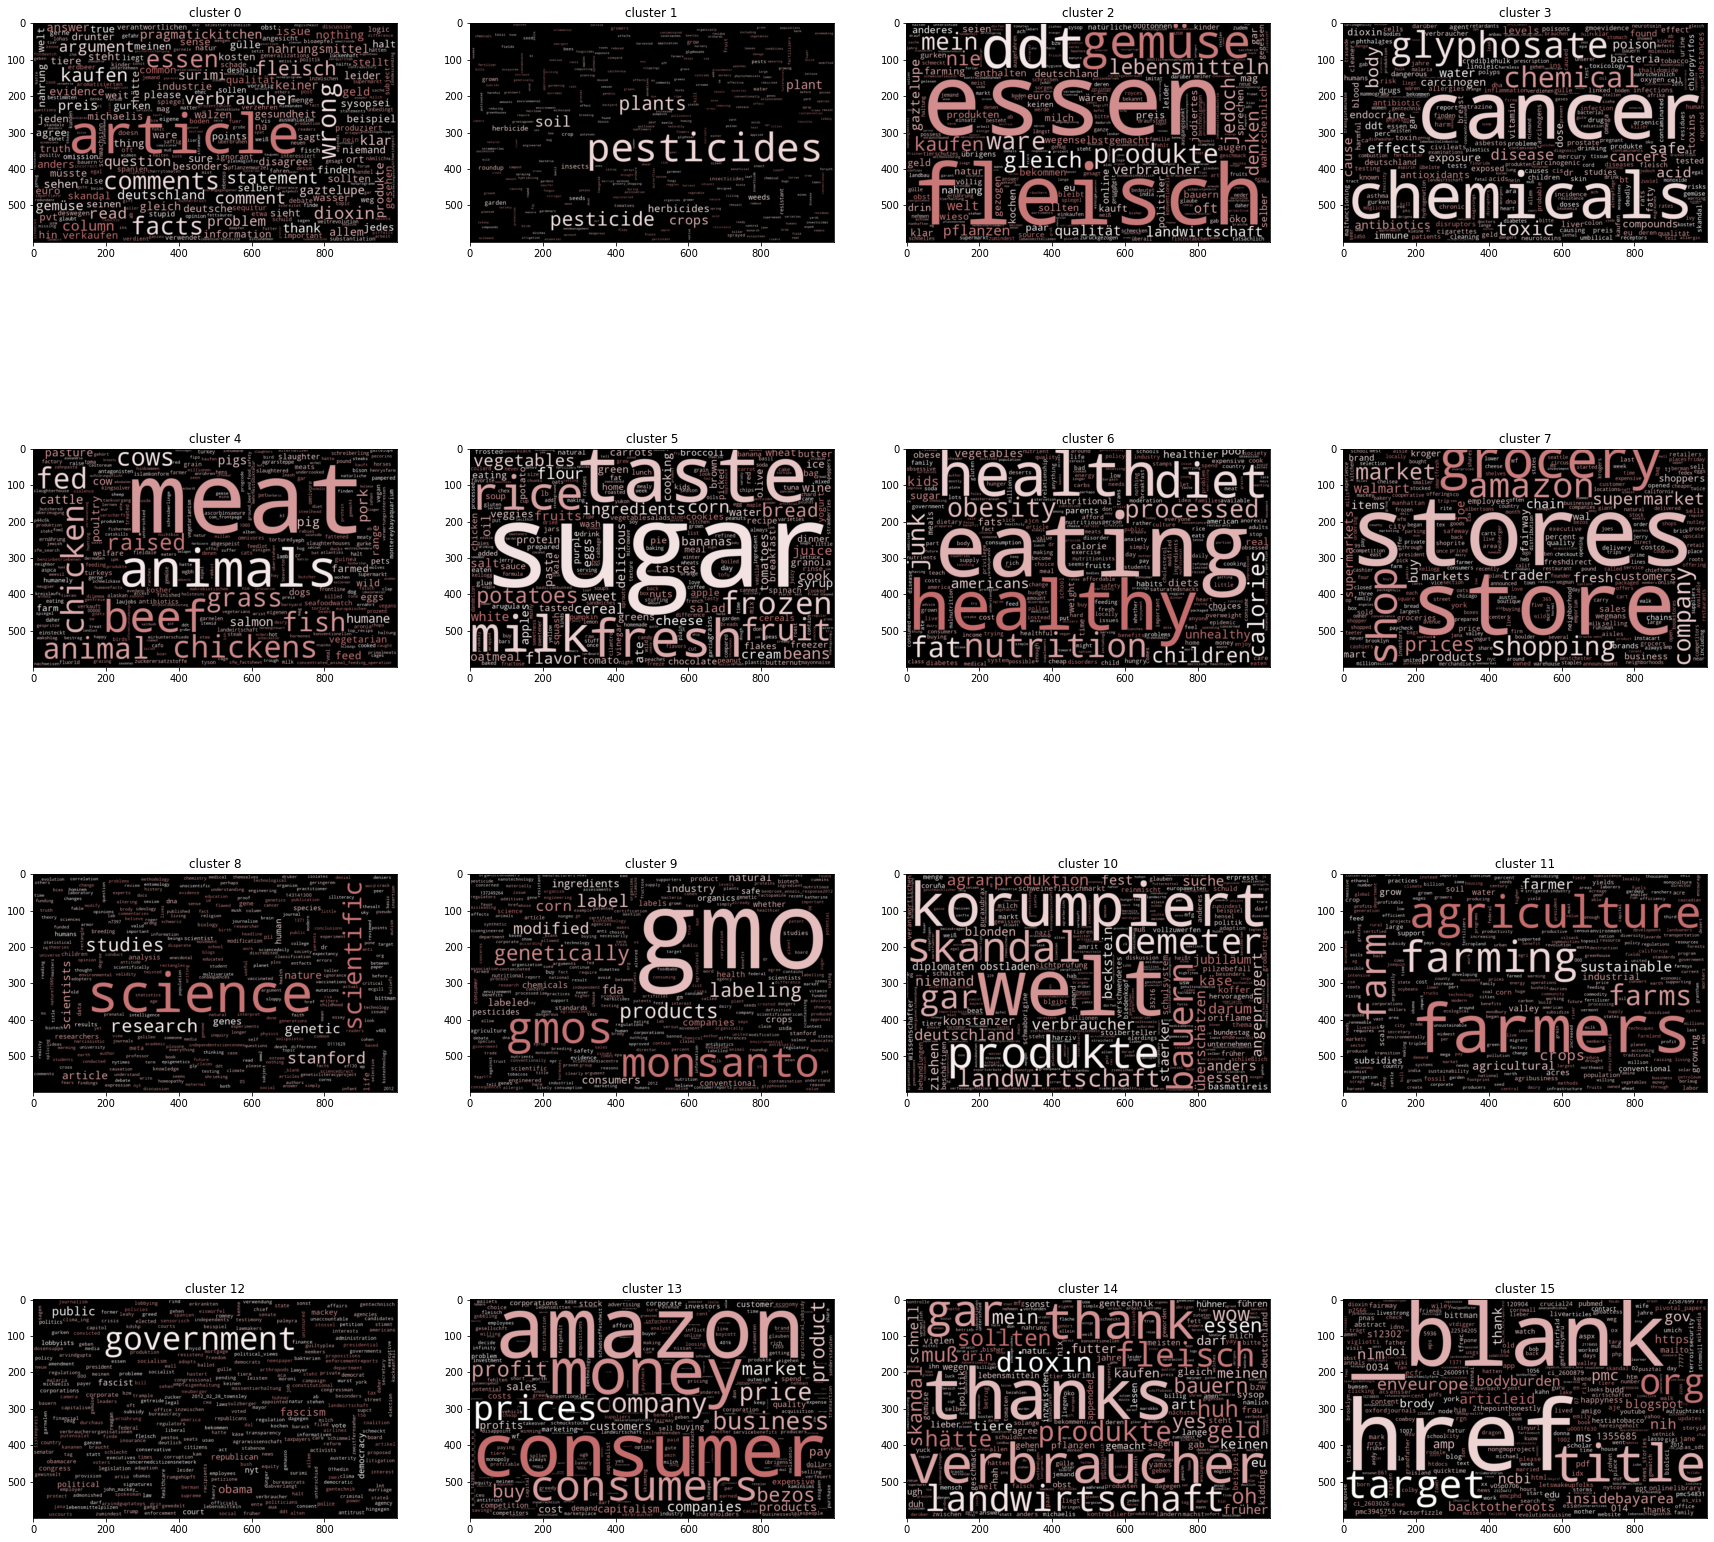
\includegraphics[width=0.3\textwidth]{images/tfhigh_wordcloud_with_full_features.png}%
  }
\end{subfloatrow}
\caption{Original methodology}
\label{PC}
\end{figure}
\footline{}
    

\begin{figure}
\floatsetup{capposition = below, floatrowsep =qquad,}

\begin{subfloatrow}
    \ffigbox[0.33\textwidth]{\caption{\small{Second methodology on English corpus: clarity scores with NLTK and sklearn stopwords}}}{%
  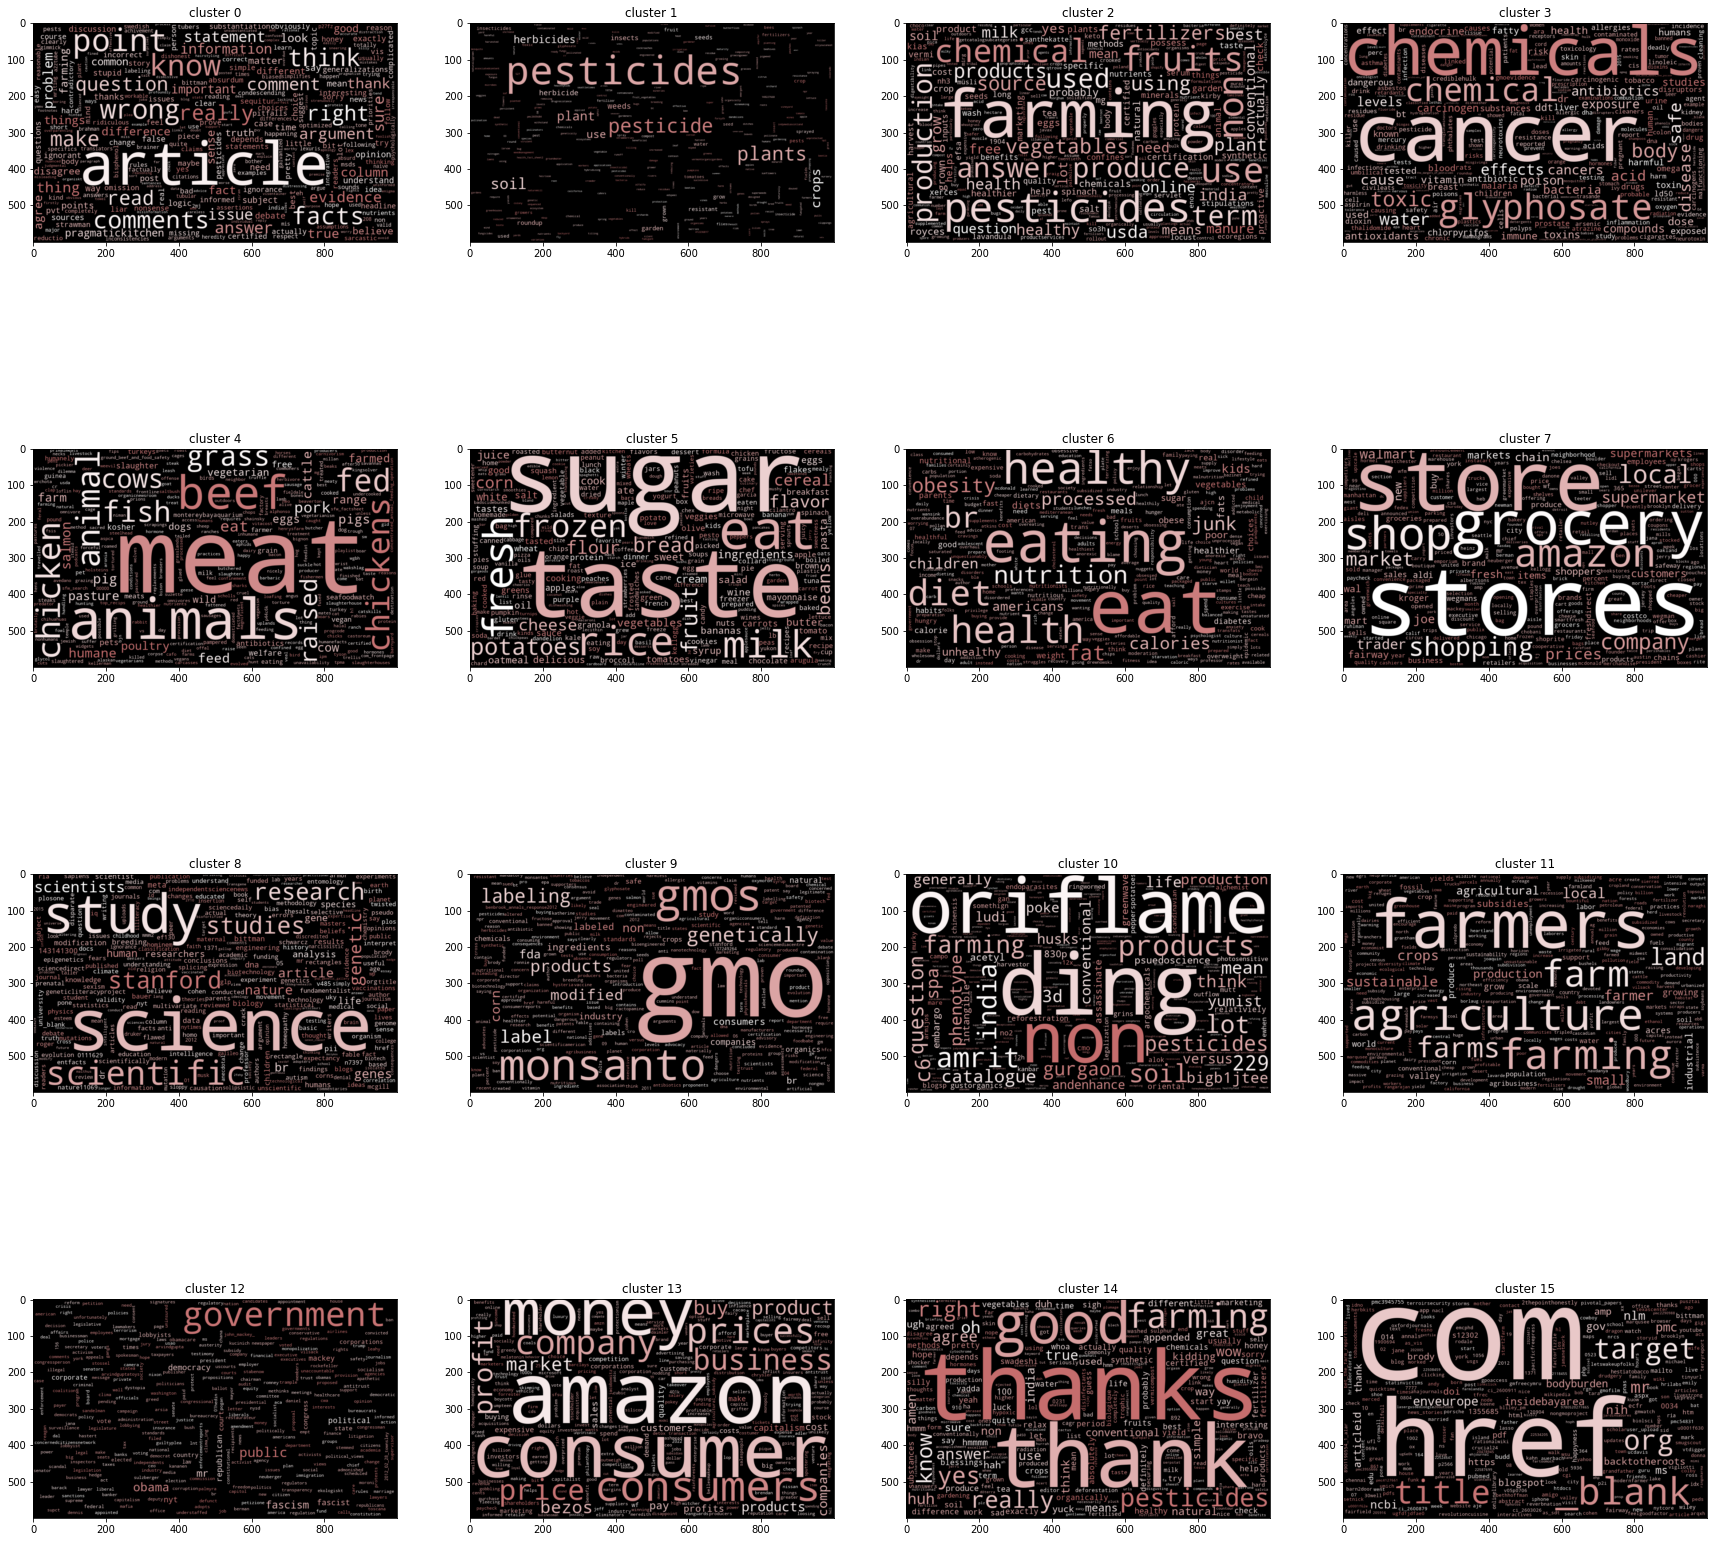
\includegraphics[width=0.3\textwidth]{images/en_nltk_sklearn_wordcloud.png}%
  }
    \ffigbox[0.33\textwidth]{\caption{\small{Second methodology on German corpus: clarity scores with NLTK and sklearn stopwords}}}{%
  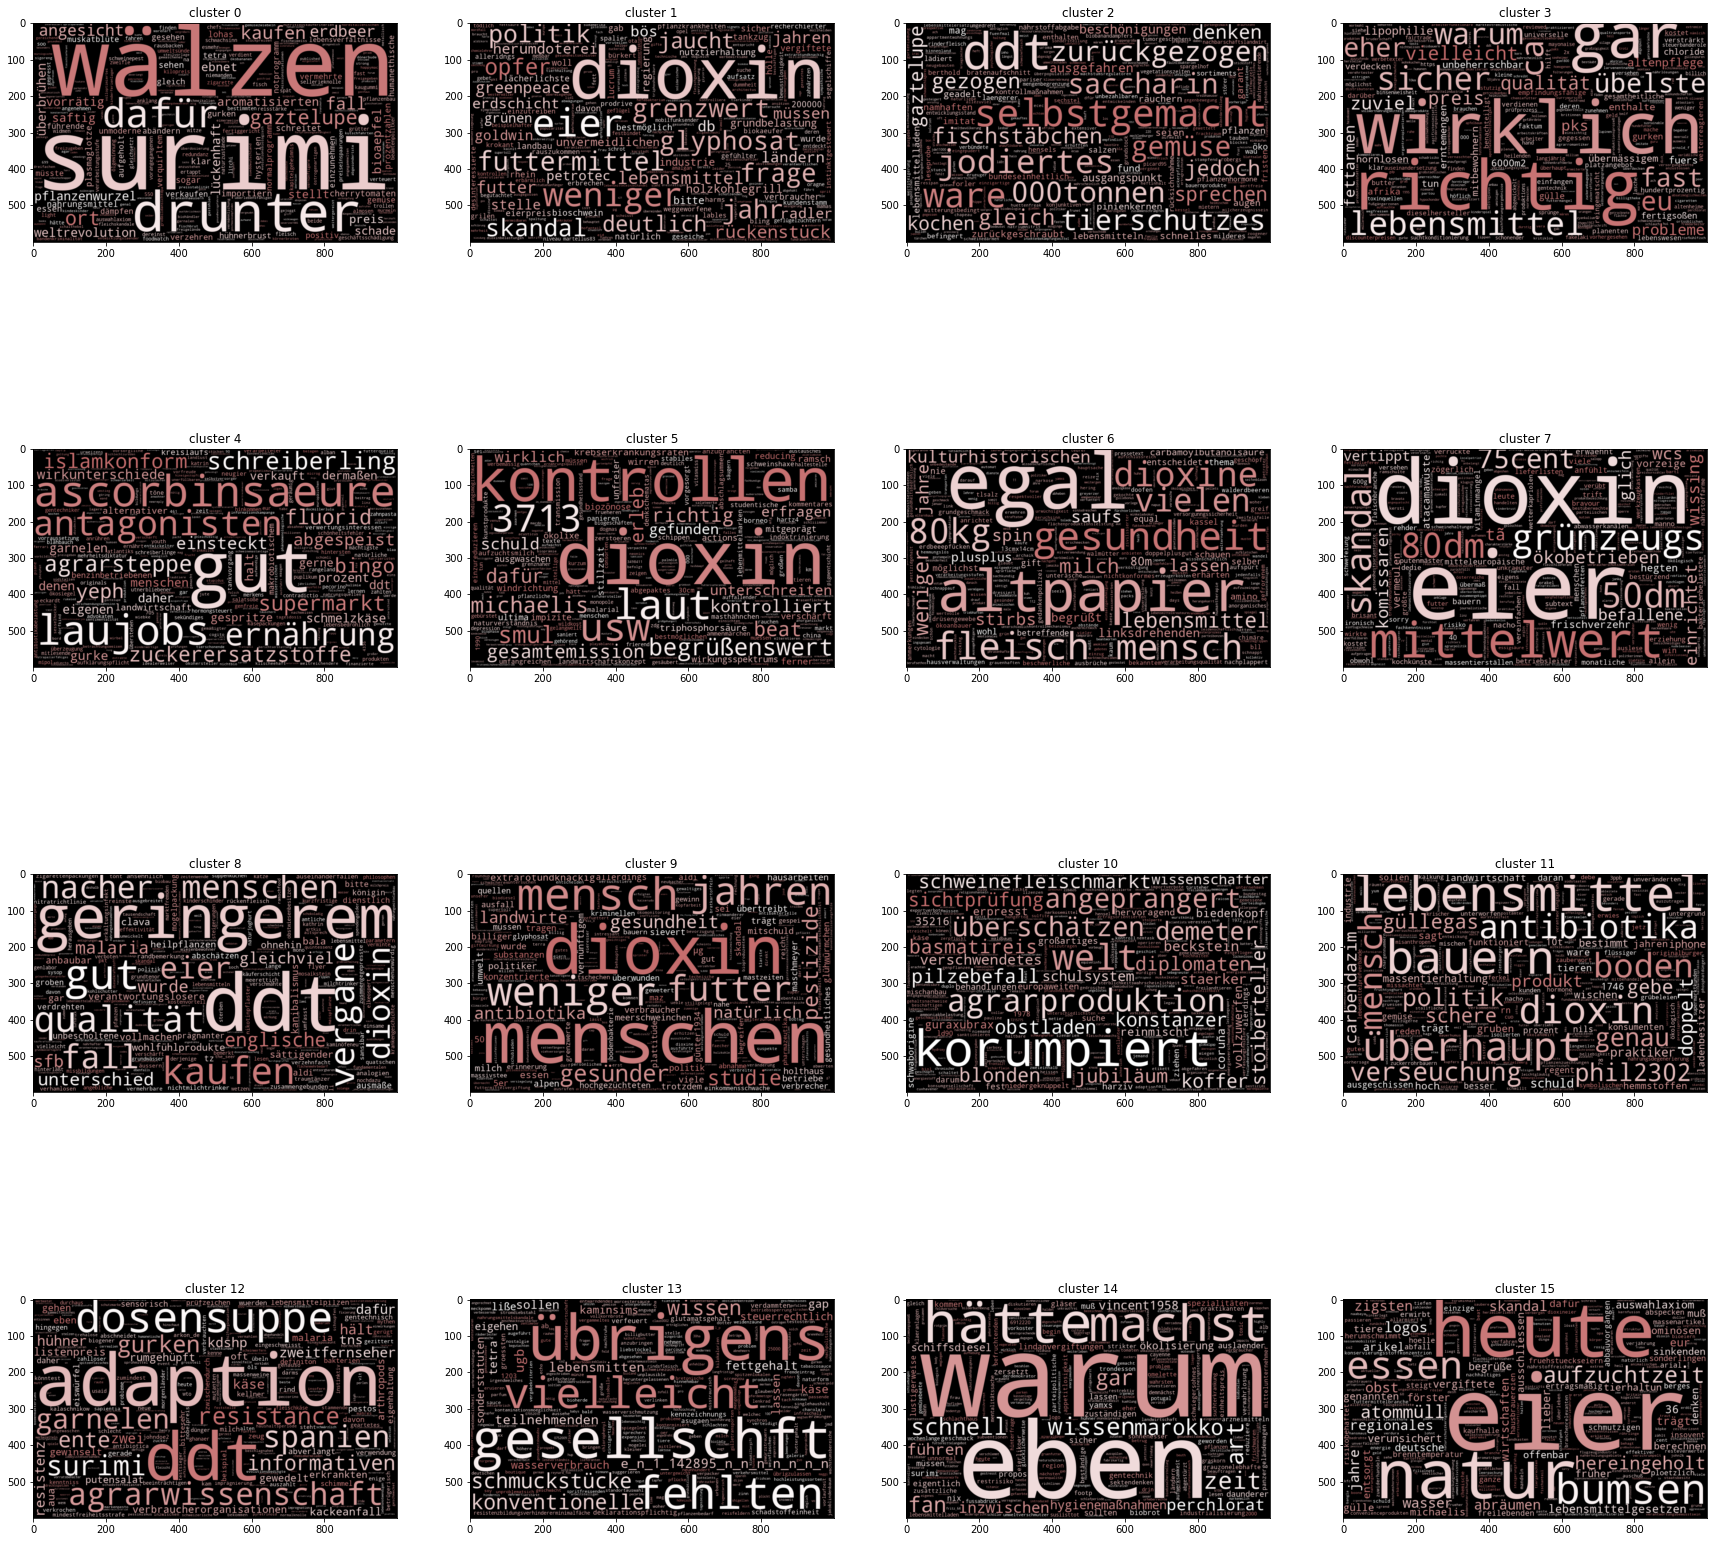
\includegraphics[width=0.3\textwidth]{images/de_nltk_sklearn_wordcloud.png}%
  }
    \ffigbox[0.33\textwidth]{\caption{\small{Top 20 words from two languages sorted by their relative clarity scores}}}{%
  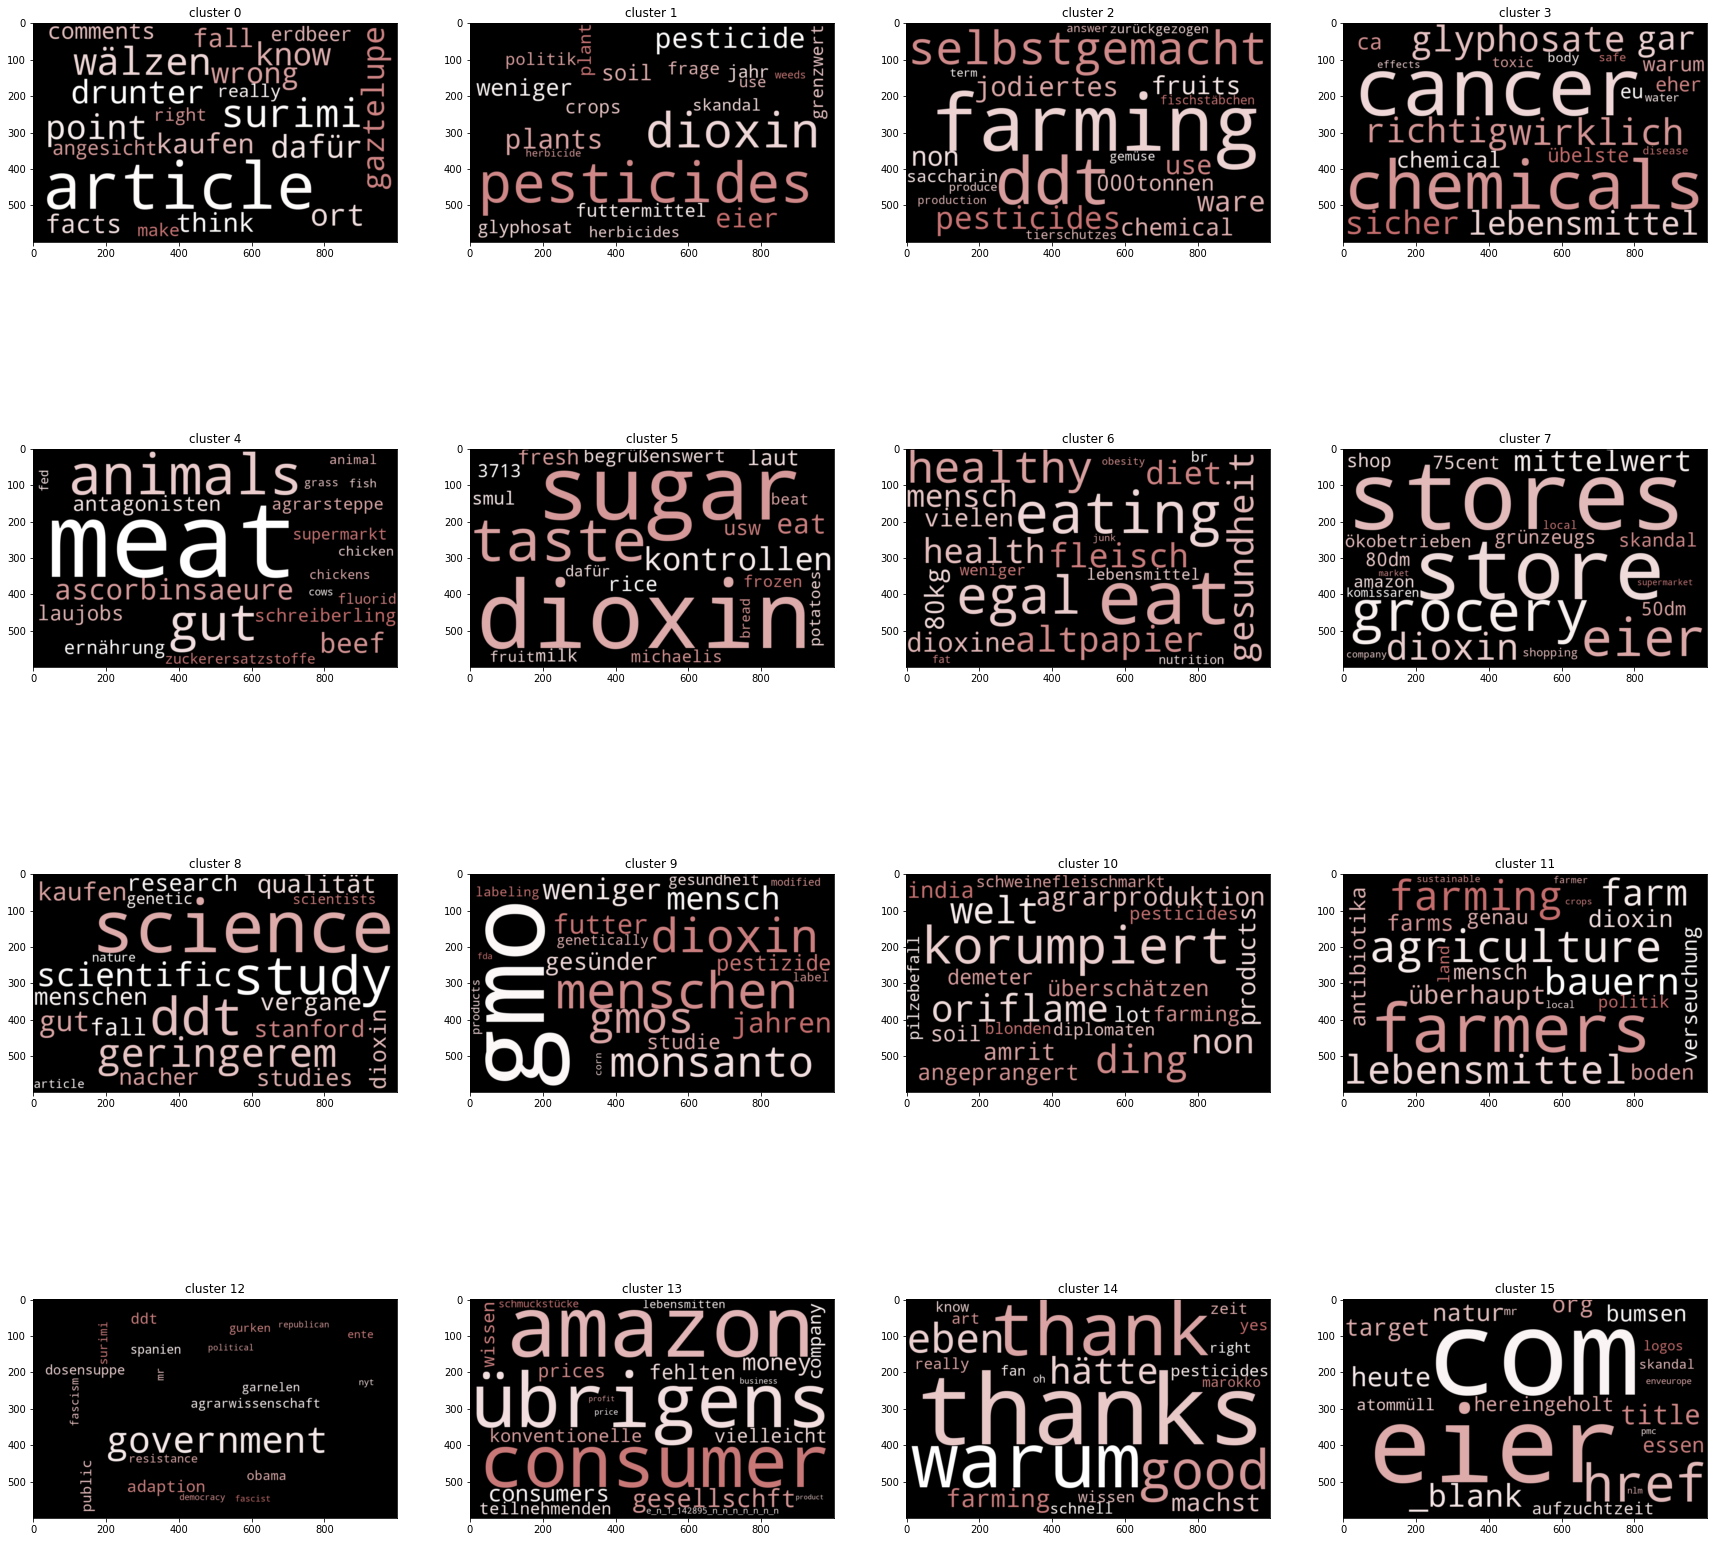
\includegraphics[width=0.3\textwidth]{images/weighted_nltk_sklearn_top20_wordcloud.png}%
  }
\end{subfloatrow}
\caption{Second methodology}
\label{PC}
\end{figure}
\footline{}


\begin{figure}
\begin{subfloatrow}
    \ffigbox[0.5\textwidth]{\caption{\small{Second methodology on English corpus: term-frequency distribution}}}{%
  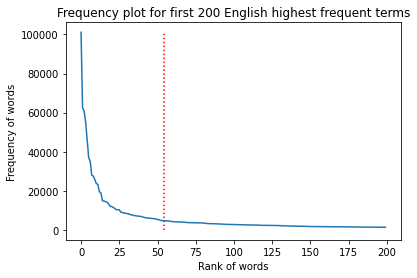
\includegraphics[width=0.5\textwidth]{images/en_tf_plot.png}%
  }
    \ffigbox[0.5\textwidth]{\caption{\small{Second methodology on German corpus: term-frequency distribution}}}{%
  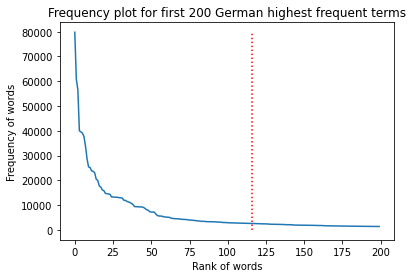
\includegraphics[width=0.5\textwidth]{images/de_tf_plot.png}%
  }
\end{subfloatrow}
\end{figure}

\begin{figure}
\floatsetup{capposition = below, floatrowsep =qquad,}
\begin{subfloatrow}
    \ffigbox[0.33\textwidth]{\caption{\small{Second methodology on English corpus: clarity scores with TF-high stopwords}}}{%
  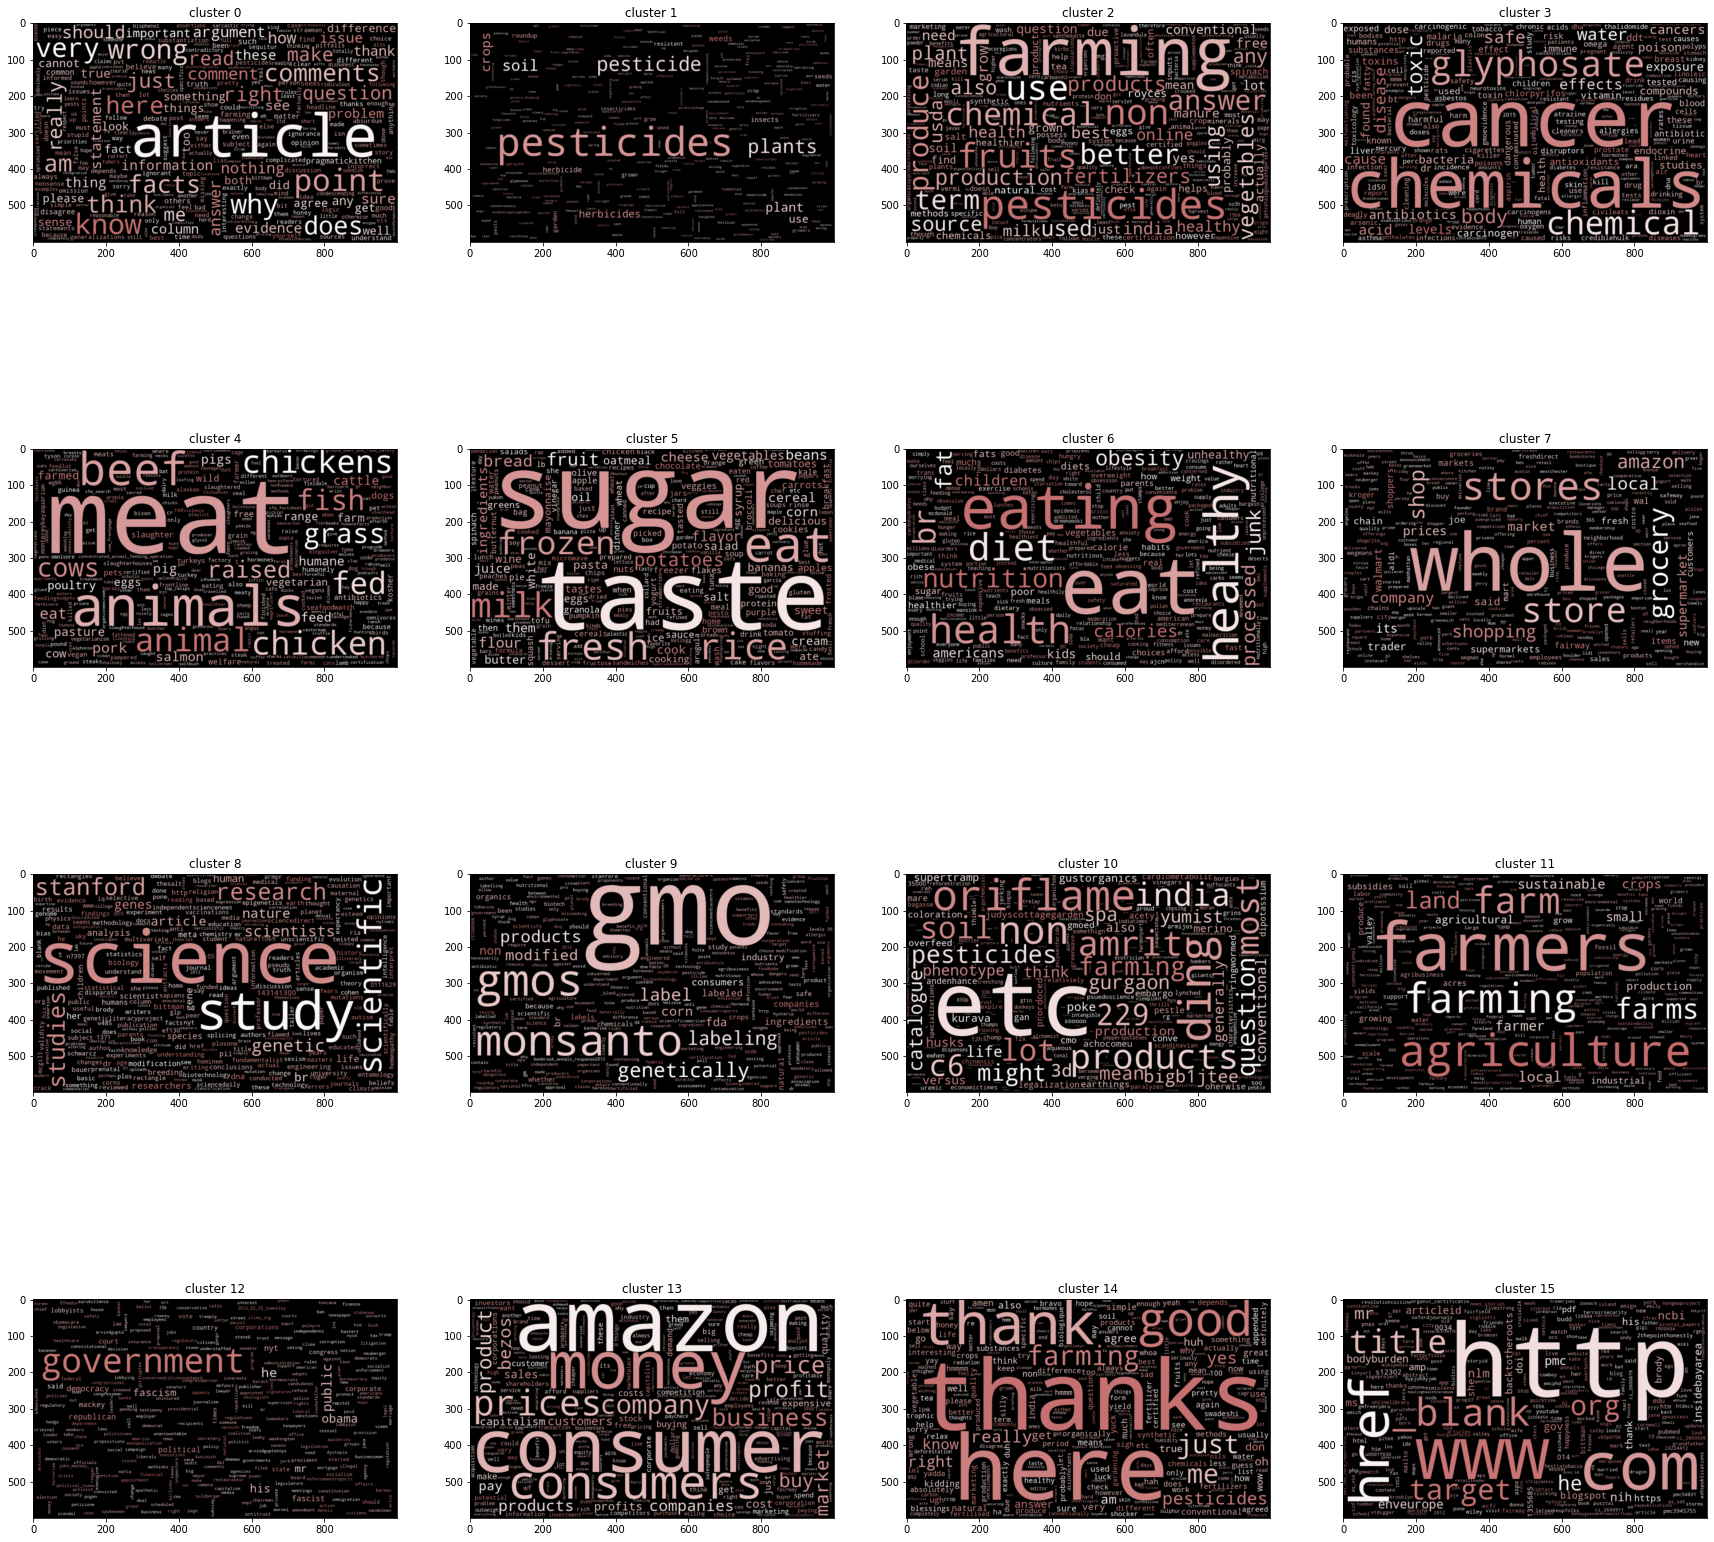
\includegraphics[width=0.3\textwidth]{images/en_tfhigh_wordcloud.png}%
  }
    \ffigbox[0.33\textwidth]{\caption{\small{Second methodology on German corpus: clarity scores with TF-High stopwords}}}{%
  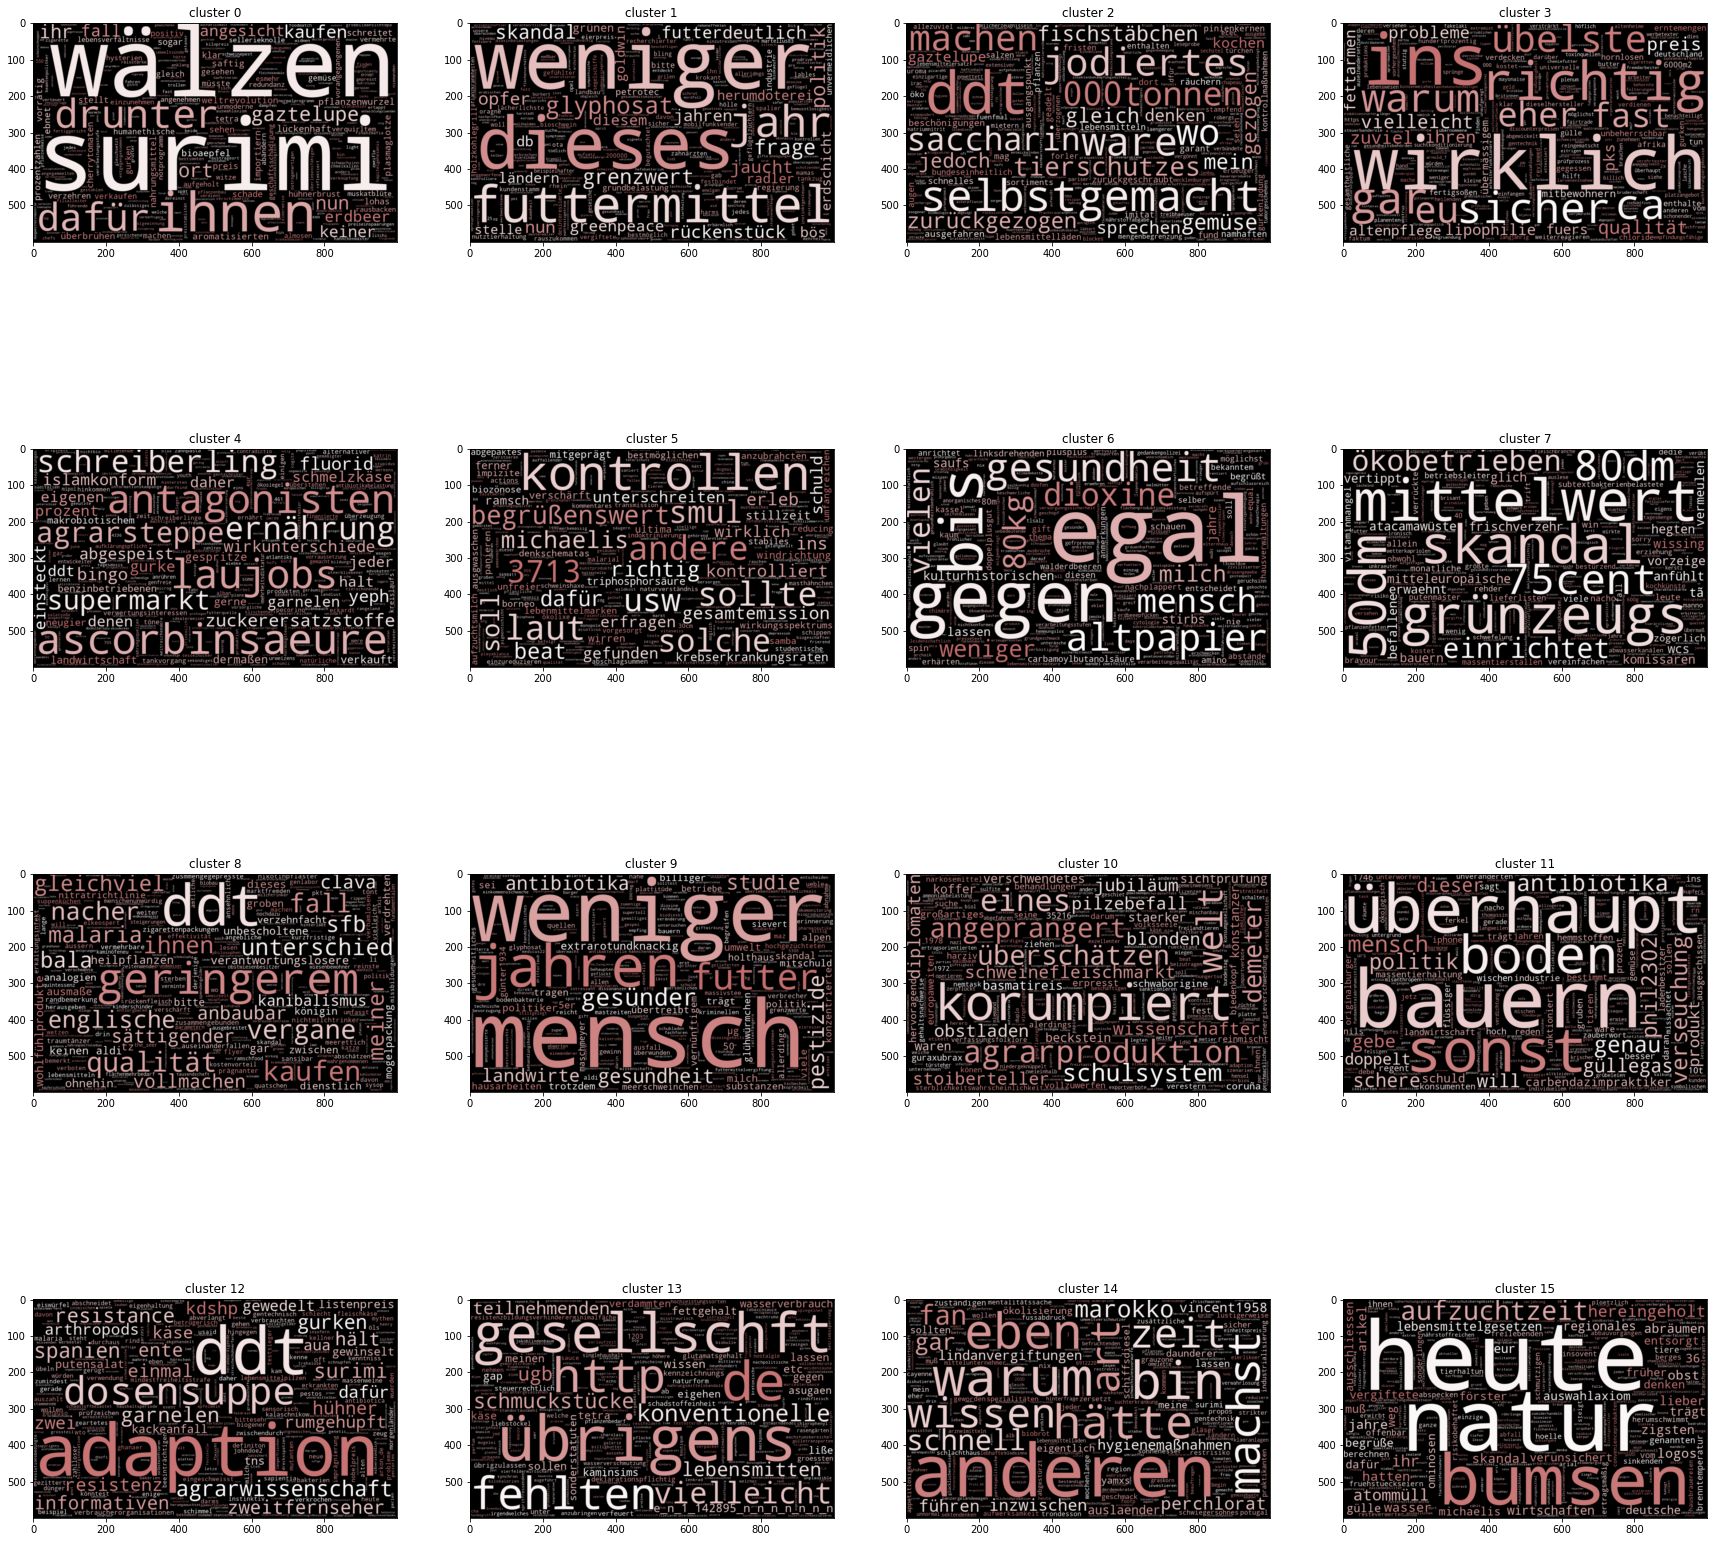
\includegraphics[width=0.3\textwidth]{images/de-tfhigh_wordcloud_116_stopwords.png}%
  }
    \ffigbox[0.33\textwidth]{\caption{\small{Top 20 words from two languages sorted by their relative clarity scores}}}{%
  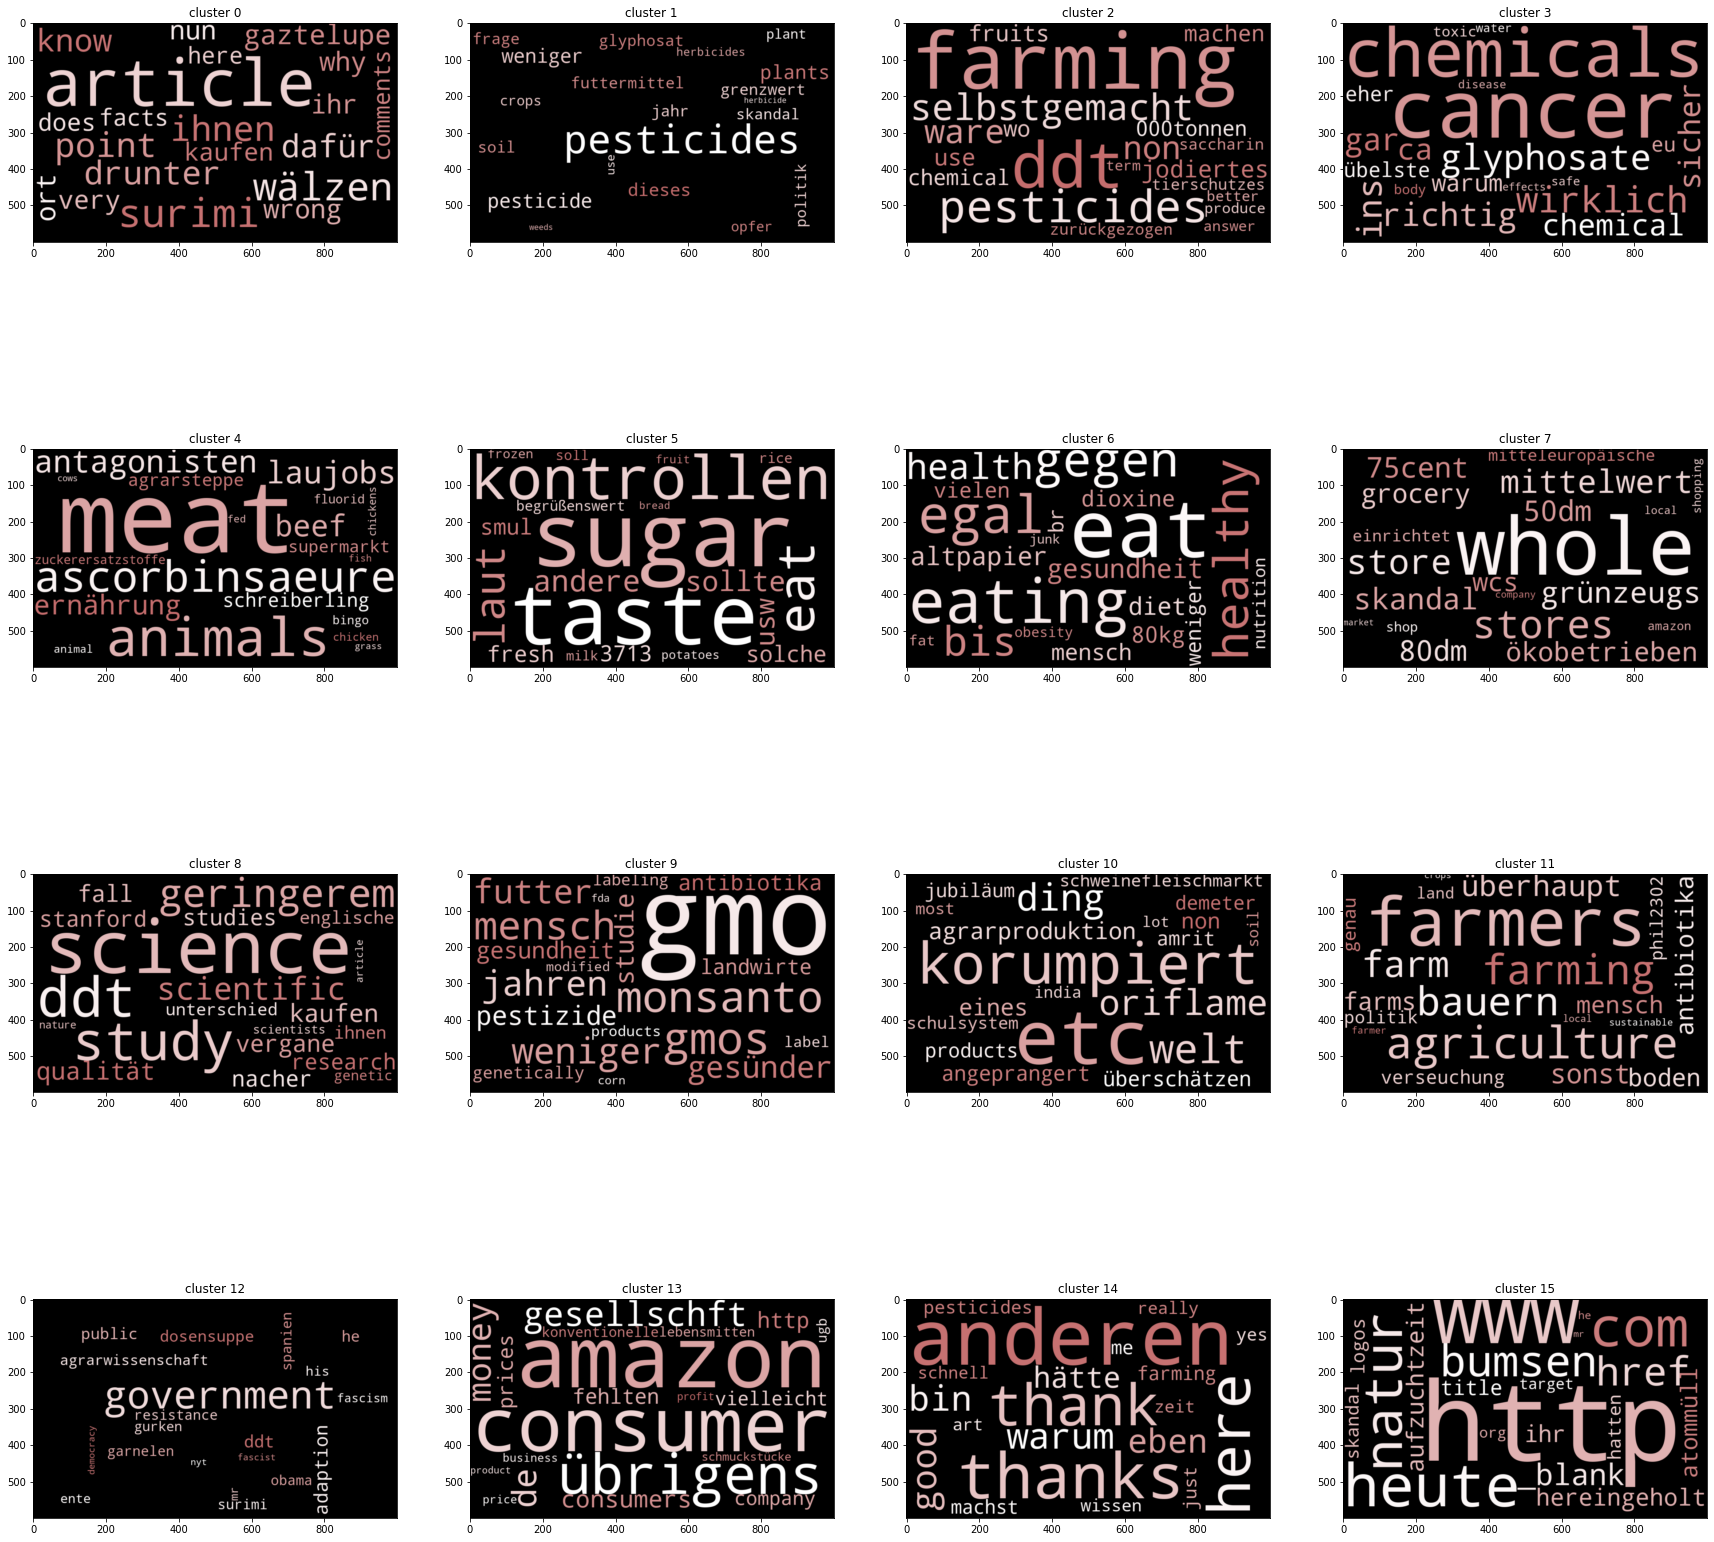
\includegraphics[width=0.3\textwidth]{images/weighted_tfhigh_top20_wordcloud_116_de_stopwords.png}%
  }
\end{subfloatrow}
\caption{Second methodology}
\label{PC}
\end{figure}
\footline{}


\begin{figure}
\floatsetup{capposition = below, floatrowsep =qquad,}
\begin{subfloatrow}
    \ffigbox[0.5\textwidth]{\caption{\small{Additional try for English corpus only: clarity scores with TF-high stopwords \\ Remarks: The cluster number is not match as shown before}}}{%
  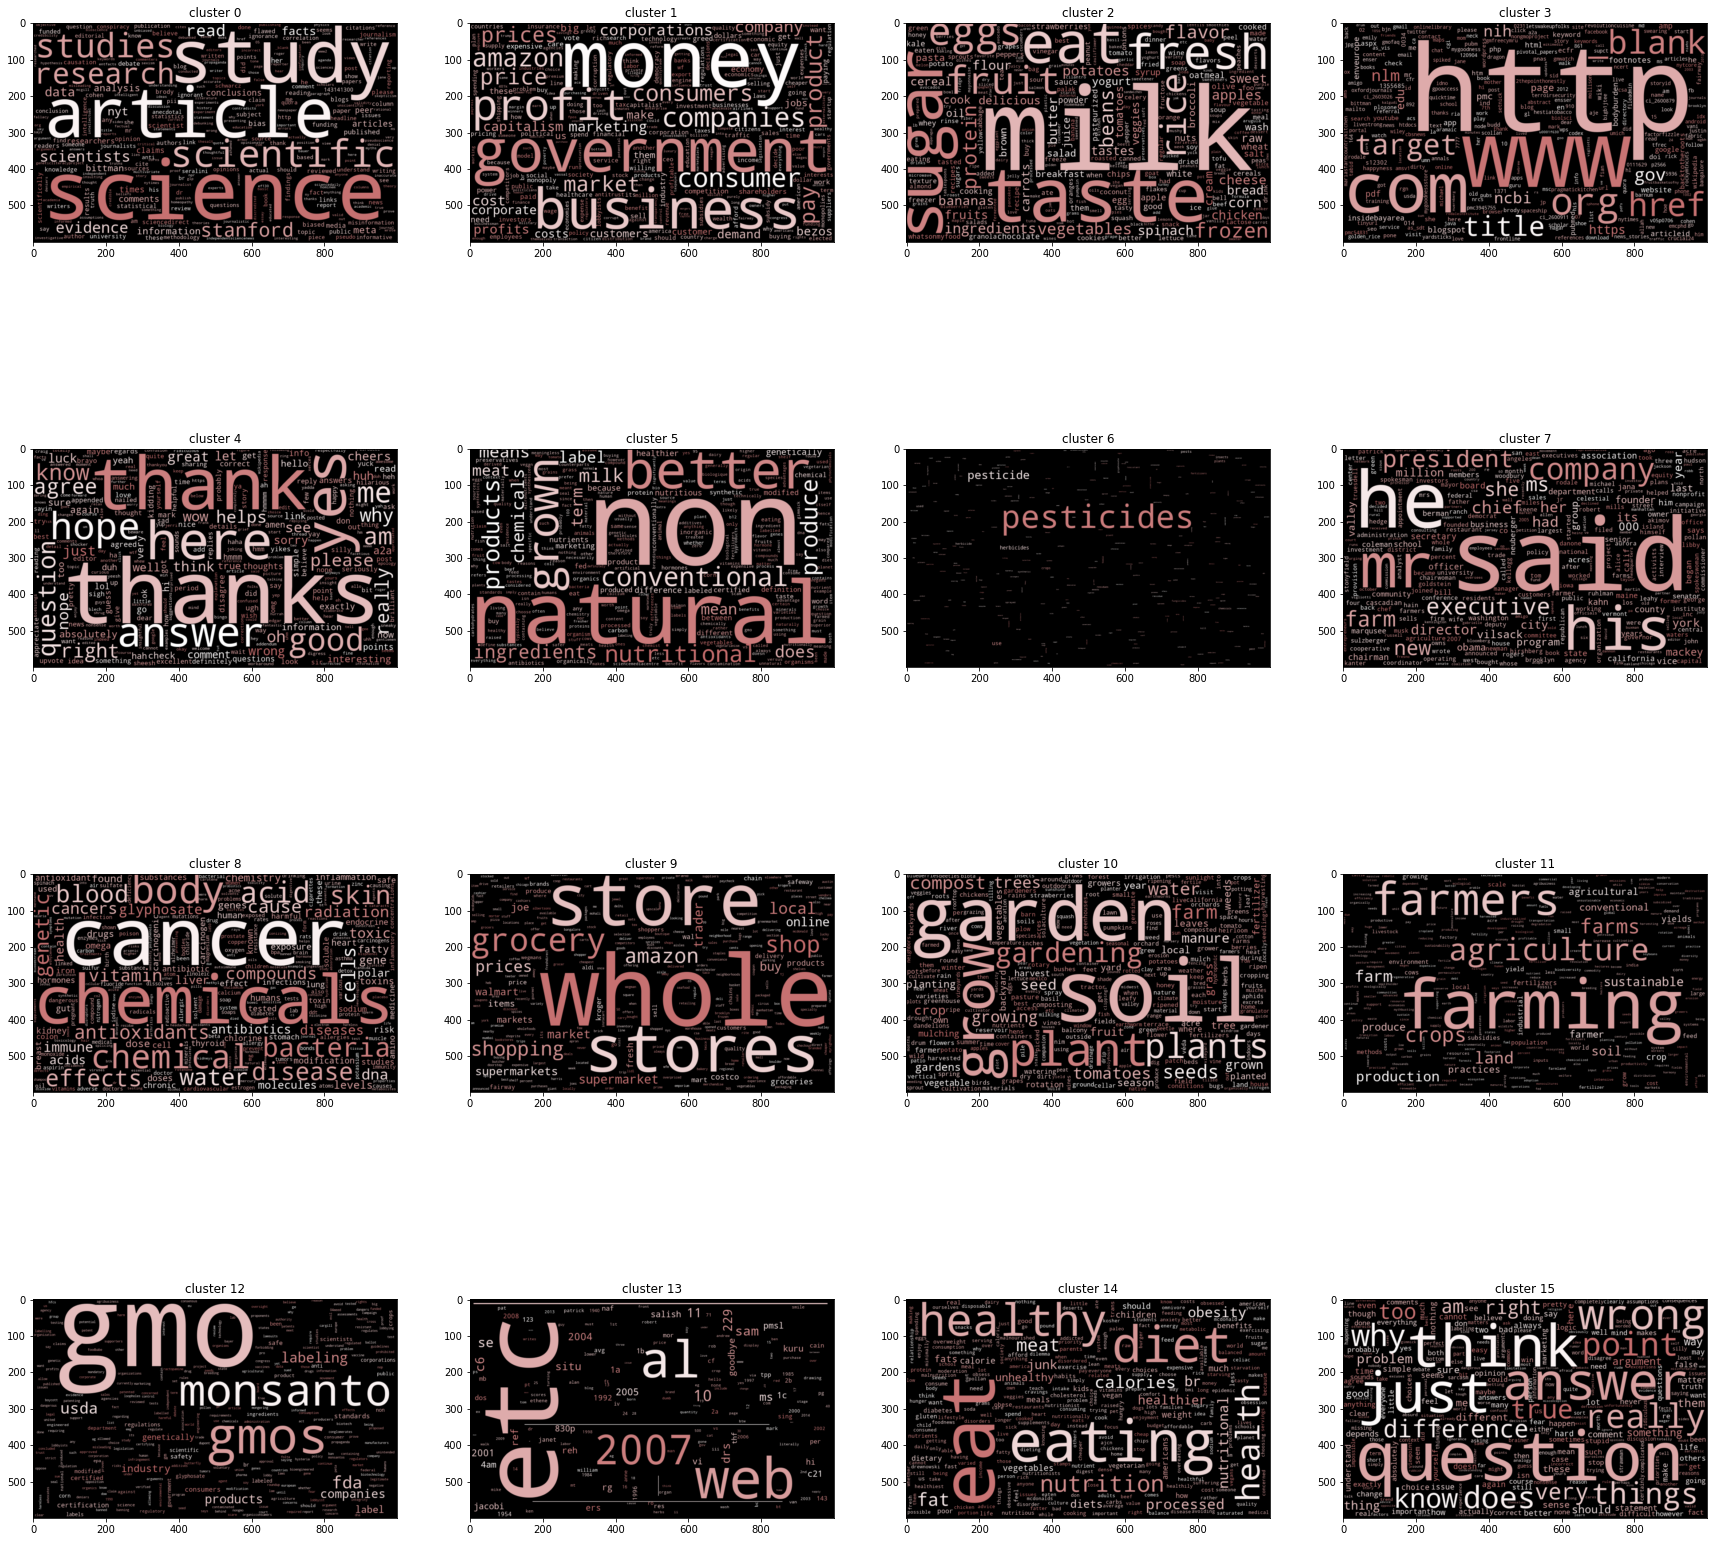
\includegraphics[width=0.4\textwidth]{images/en_tfhigh_kmean_for_en_only.png}%
  }
    \ffigbox[0.5\textwidth]{\caption{\small{Additional try for German corpus only: clarity scores with TF-high stopwords \\ Remarks: The cluster number is not match as shown before}}}{%
  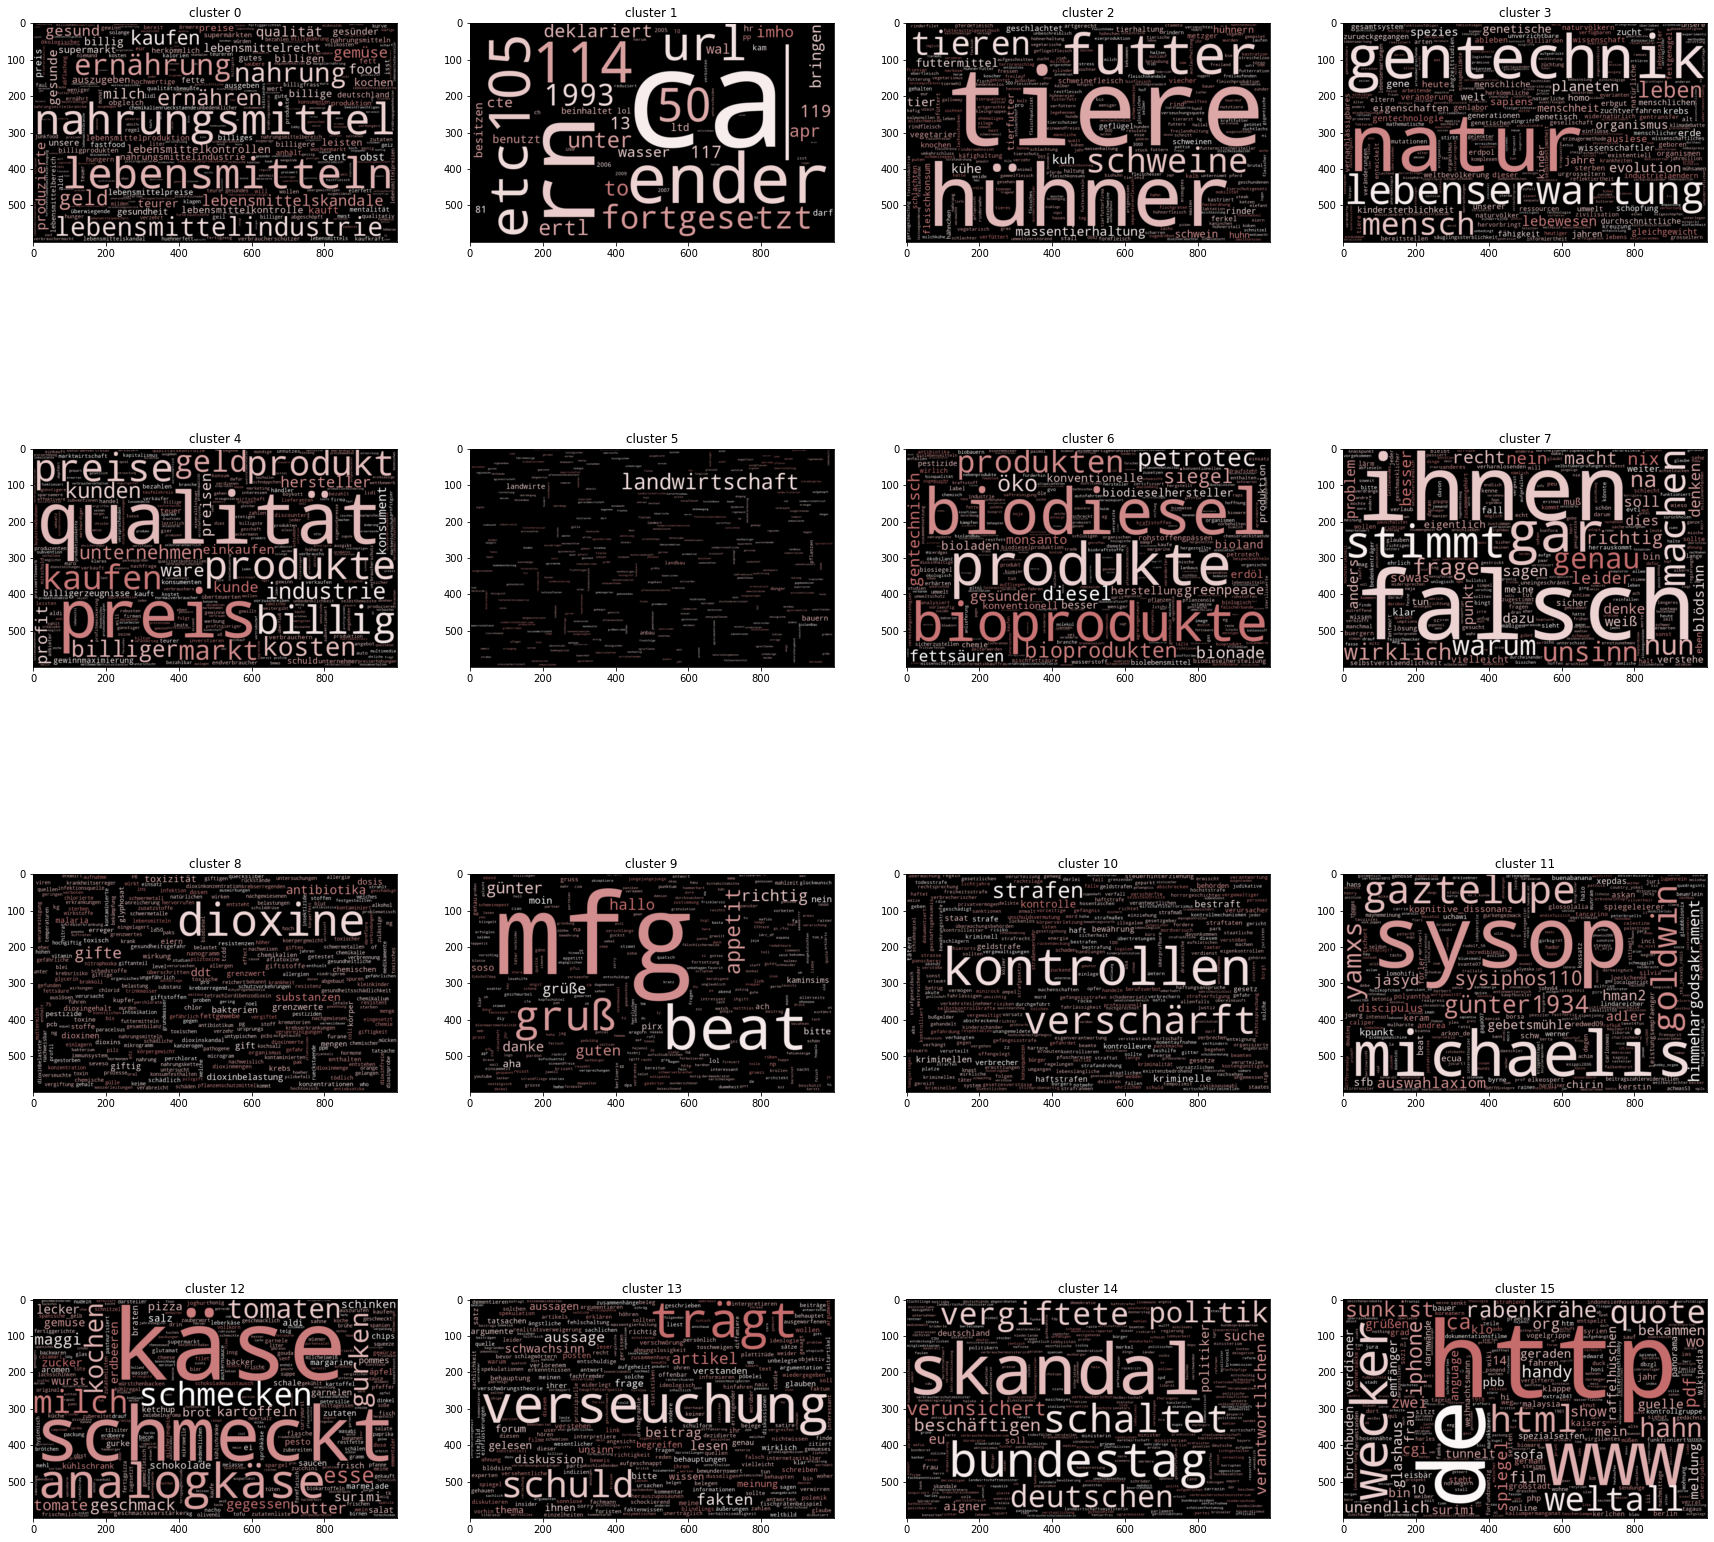
\includegraphics[width=0.4\textwidth]{images/de_tfhigh_116_stopwords_kmean_for_de_only.png}%
  }
\end{subfloatrow}
\caption{Additional try}
\label{PC}
\end{figure}
\footline{}

\begin{figure}
\floatsetup{capposition = below, floatrowsep =qquad,}
\begin{subfloatrow}
    \ffigbox[0.5\textwidth]{\caption{\small{Additional try for English corpus only: embedding distribution \\ Remarks: The cluster number is not match as shown before}}}{%
  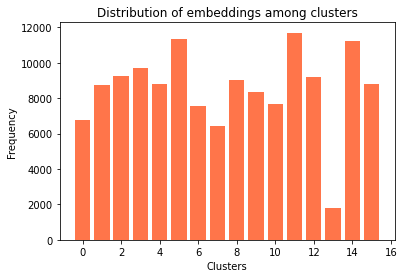
\includegraphics[width=0.4\textwidth]{images/16ks-en-bar.png}%
  }
    \ffigbox[0.5\textwidth]{\caption{\small{Additional try for German corpus only:embedding distribution \\ Remarks: The cluster number is not match as shown before}}}{%
  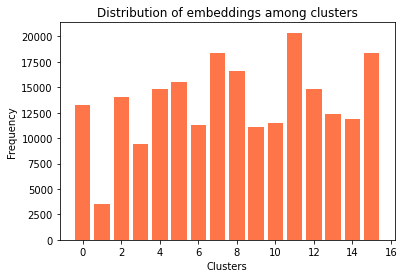
\includegraphics[width=0.4\textwidth]{images/16ks-de-bar.png}%
  }
\end{subfloatrow}
\caption{Additional try}
\label{PC}
\end{figure}
\footline{}

\end{document}
